\section{Proof of the main theorem}\label{sec:proof}

In this section, we present the proof of our main Theorem~\ref{thm:h62}. 

\begin{theorem}[Theorem~\ref{thm:h62}] \label{thm:126survives}
    \uses{thm:bjmbx,prop:possibleh62,prop:state5false}
    \lean{KervaireInvariant.MainProof.theorem_126survives}
    The element $h_6^2$ survives to the $E_\infty$-page in the Adams spectral sequence.
\end{theorem}

We first recall the following theorem, known as the inductive method, originally by Barratt--Jones--Mahowald \cite{BJMinduction} and later extended to the H$\mathbb{F}_2$-synthetic setting by Burklund--Xu \cite[Proposition~7.19]{BurklundXu}.

\begin{notation}
    Let $\theta_5 = [h_5^2]$ represent any synthetic homotopy class in $\pi_{62,62+2}S^{0,0}$ detected by $h_5^2$ in the Adams $E_2$-page. For convenience, we use the same notation, $\theta_5$, to denote its image in $\pi_{62,62+2}S^{0,0}/\lambda^r$ via the map $S^{0,0} \rightarrow S^{0,0}/\lambda^r$ for all $r \ge 1$. Similarly, let $\eta = [h_1] \in \pi_{1,1+1}S^{0,0}$.
\end{notation}


\begin{axiom}[Barratt--Jones--Mahowald, Burklund--Xu] \label{thm:bjmbx}
\lean{KervaireInvariant.MainProof.theorem_bjmbx}
\begin{enumerate}
 \item[]
 \item    The element $h_6^2$ survives to the $E_{r+3}$-page of the classical Adams spectral sequence if and only if for some $\theta_5$, 
 $$\lambda \eta \theta_5^2 = 0 \ \text{in} \ \pi_{125,125+4} S^{0,0}/\lambda^{r+1}.$$
 \item   In particular, $h_6^2$ is a permanent cycle in the classical Adams spectral sequence if and only if for some $\theta_5$,
 $$\lambda \eta \theta_5^2 = 0 \ \text{in} \ \pi_{125,125+4} S^{0,0}.$$ 
 \end{enumerate}
\end{axiom}

\begin{remark}
    The statement in Axiom~\ref{thm:bjmbx}(1) was originally stated as 
    $$\eta \theta_5^2 = 0 \ \text{in} \ \pi_{125,125+5} S^{0,0}/\lambda^r$$
    in \cite[Proposition~7.19]{BurklundXu}. Upon inspection, $\pi_{125,125+5} S^{0,0}$ doesn't contain any $\lambda$-torsion classes, so this is equivalent to the version we stated, which is more consistent with the statement in part (2). 
\end{remark}

\begin{remark} \label{rem:theta5choice}
    \lean{KervaireInvariant.MainProof.remark_theta5choice}
    Axiom~\ref{thm:bjmbx} is proved using the quadratic construction  on a map from the mod 2 Moore spectrum to the sphere spectrum, where the restriction on the bottom cell is $\theta_5$. Therefore, it is necessary to use a $\theta_5$ of order 2. 
    
    Notably, \cite{Xu, IWX} confirms that all classical $\theta_5$'s indeed have order 2. Furthermore, from Proposition~\ref{prereq:prop:syn-einfty-nuX} and an analysis of the differentials in the classical Adams spectral sequence, we find that $\pi_{62,62+2}S^{0,0}$ doesn't contain any $\lambda$-torsion. Consequently, all synthetic $\theta_5$'s also have order 2, making it valid to apply Axiom~\ref{thm:bjmbx} to any $\theta_5$. 
    
    Additionally, since the proof of Axiom~\ref{thm:bjmbx} shows that the expression $\lambda \eta \theta_5^2$ corresponds to the total differential $\delta_1: S^{0,0}/\lambda \rightarrow S^{1,-1}$ on $h_6^2$, the value of the expression $\lambda \eta \theta_5^2$ is consistent for every choice of $\theta_5$.  (Note that our grading for the triangulation translation functor is smashing with $S^{1,0}$, which is consistent with \cite[Appendix A]{BHS} but is different from \cite[Section 7]{BurklundXu}, so the target of $\delta_1$ is $S^{1,-1}$. )
\end{remark}

We pay special attention to the following three elements on the classical Adams $E_2$-page (see Figure~\ref{Fig:near126} and Tables~\ref{Table:S125.19}, \ref{Table:S126.10}, \ref{Table:S124.12}, \ref{Table:S125.20} in the Appendix): 
\begin{align*}
    h_1h_4x_{109,12} & \in \Ext_A^{14, 125+14}, \\
    x_{126,8,4} + x_{126,8} & \in \Ext_A^{8, 126+8}, \\
    h_0^2x_{124,8} & \in \Ext_A^{10, 124+10},\\
    g^4\Delta h_1g & \in \Ext_A^{25,125+25}.
\end{align*}

For the right side of Figure ~\ref{Fig:near126}, we use dashed differentials to indicate the shortest possible nonzero differentials that these elements could support.

{

\newcommand{\labelar}[1]{\overset{\uparrow}{#1}}
\newdimen\widthA\newcommand{\resizelabel}[2]{\settowidth{\widthA}{#2}\pgfmathsetmacro{\ratio}{min((1cm)/max(\widthA, 1cm), #1)}\scalebox{\ratio}{#2}}

\begin{figure}
\centering
\scalebox{1}{
\begin{tikzpicture}[line width=0.1pt]
\draw (121.5,-0.5) rectangle (127.5,19.5);
\node at (122,-1) {$122$};
\node at (123,-1) {$123$};
\node at (124,-1) {$124$};
\node at (125,-1) {$125$};
\node at (126,-1) {$126$};
\node at (127,-1) {$127$};
\node at (121,0) {$0$};
\node at (121,1) {$1$};
\node at (121,2) {$2$};
\node at (121,3) {$3$};
\node at (121,4) {$4$};
\node at (121,5) {$5$};
\node at (121,6) {$6$};
\node at (121,7) {$7$};
\node at (121,8) {$8$};
\node at (121,9) {$9$};
\node at (121,10) {$10$};
\node at (121,11) {$11$};
\node at (121,12) {$12$};
\node at (121,13) {$13$};
\node at (121,14) {$14$};
\node at (121,15) {$15$};
\node at (121,16) {$16$};
\node at (121,17) {$17$};
\node at (121,18) {$18$};
\node at (121,19) {$19$};
\begin{scope}
\clip (121.5,-0.5) rectangle (127.5,19.5);
\draw[black!10] (122.5,-0.5) -- (122.5,19.5);
\draw[black!10] (123.5,-0.5) -- (123.5,19.5);
\draw[black!10] (124.5,-0.5) -- (124.5,19.5);
\draw[black!10] (125.5,-0.5) -- (125.5,19.5);
\draw[black!10] (126.5,-0.5) -- (126.5,19.5);
\draw[black!10] (121.5,0.5) -- (127.5,0.5);
\draw[black!10] (121.5,1.5) -- (127.5,1.5);
\draw[black!10] (121.5,2.5) -- (127.5,2.5);
\draw[black!10] (121.5,3.5) -- (127.5,3.5);
\draw[black!10] (121.5,4.5) -- (127.5,4.5);
\draw[black!10] (121.5,5.5) -- (127.5,5.5);
\draw[black!10] (121.5,6.5) -- (127.5,6.5);
\draw[black!10] (121.5,7.5) -- (127.5,7.5);
\draw[black!10] (121.5,8.5) -- (127.5,8.5);
\draw[black!10] (121.5,9.5) -- (127.5,9.5);
\draw[black!10] (121.5,10.5) -- (127.5,10.5);
\draw[black!10] (121.5,11.5) -- (127.5,11.5);
\draw[black!10] (121.5,12.5) -- (127.5,12.5);
\draw[black!10] (121.5,13.5) -- (127.5,13.5);
\draw[black!10] (121.5,14.5) -- (127.5,14.5);
\draw[black!10] (121.5,15.5) -- (127.5,15.5);
\draw[black!10] (121.5,16.5) -- (127.5,16.5);
\draw[black!10] (121.5,17.5) -- (127.5,17.5);
\draw[black!10] (121.5,18.5) -- (127.5,18.5);
  \draw (127,1) -- (127,2);
  \draw (127,1) -- (128,2);
  \draw (127,1) -- (130,2);
  \draw (126,2) -- (126,3);
  \draw (126,2) -- (127.112,2.959);
  \draw (126,2) -- (128.888,3.041);
  \draw (120.892,7.039) -- (122,8);
  \draw (127,2) -- (126.888,3.041);
  \draw (127,2) -- (130,3);
  \draw (126,3) -- (126.097,3.965);
  \draw (126,3) -- (129,4);
  \draw (120,9) -- (123.134,9.951);
  \draw (127.112,2.959) -- (128,4);
  \draw (126.888,3.041) -- (127,4);
  \draw (126.888,3.041) -- (130,4);
  \draw (126.097,3.965) -- (126,5);
  \draw (126.097,3.965) -- (129.143,4.948);
  \draw (125.903,4.035) -- (129,5);
  \draw (125,5) -- (124.935,6.024);
  \draw (125,5) -- (128.162,5.941);
  \draw (125,5) -- (127.838,6.059);
  \draw (124,6) -- (124.139,6.949);
  \draw (124,6) -- (125,7);
  \draw (124,6) -- (127.178,6.935);
  \draw (124,6) -- (127.089,6.968);
  \draw (120.901,9.036) -- (123.769,10.084);
  \draw (120.158,9.942) -- (123.244,10.911);
  \draw (119.842,10.058) -- (122.756,11.089);
  \draw (118.932,11.025) -- (122.139,11.949);
  \draw (118.932,11.025) -- (122,12);
  \draw (118.796,11.074) -- (122.139,11.949);
  \draw (127,4) -- (127,5);
  \draw (126,5) -- (126.055,5.98);
  \draw (125.065,5.976) -- (125.953,7.017);
  \draw (125.065,5.976) -- (128,7);
  \draw (124.935,6.024) -- (125,7);
  \draw (124.935,6.024) -- (128.095,6.965);
  \draw (124.139,6.949) -- (127.163,7.941);
  \draw (124,7) -- (127.081,7.97);
  \draw (123.861,7.051) -- (127,8);
  \draw (123,8) -- (122.931,9.025);
  \draw (123,8) -- (125.955,9.016);
  \draw (123,8) -- (125.775,9.082);
  \draw (119.865,11.049) -- (122.866,12.049);
  \draw (119.135,11.951) -- (122.168,12.939);
  \draw (127,5) -- (126.946,6.02);
  \draw (126.055,5.98) -- (126.047,6.983);
  \draw (125.945,6.02) -- (127.089,6.968);
  \draw (125.945,6.02) -- (129,7);
  \draw (124,8) -- (123.882,9.043);
  \draw (124,8) -- (127.178,8.935);
  \draw (124,8) -- (127.089,8.968);
  \draw (124,8) -- (127,9);
  \draw (124,8) -- (126.911,9.032);
  \draw (123.069,8.975) -- (123.134,9.951);
  \draw (123.069,8.975) -- (124.231,9.916);
  \draw (123.069,8.975) -- (123.884,10.042);
  \draw (123.069,8.975) -- (126.199,9.928);
  \draw (123.069,8.975) -- (125.901,10.036);
  \draw (122.931,9.025) -- (125.901,10.036);
  \draw (121,11) -- (124.237,11.914);
  \draw (121,11) -- (123.763,12.086);
  \draw (119.878,12.044) -- (123.138,12.95);
  \draw (127.054,5.98) -- (127.178,6.935);
  \draw (127.054,5.98) -- (128.095,6.965);
  \draw (126.946,6.02) -- (126.822,7.065);
  \draw (126.047,6.983) -- (126.219,7.92);
  \draw (125.051,7.982) -- (125.955,9.016);
  \draw (125.051,7.982) -- (128,9);
  \draw (124.949,8.018) -- (124.801,9.072);
  \draw (124.949,8.018) -- (126.045,8.984);
  \draw (124.118,8.957) -- (123.884,10.042);
  \draw (124.118,8.957) -- (123.769,10.084);
  \draw (124.118,8.957) -- (127.147,9.947);
  \draw (123.882,9.043) -- (123.884,10.042);
  \draw (123.882,9.043) -- (127.049,9.982);
  \draw (123.134,9.951) -- (123.244,10.911);
  \draw (123.134,9.951) -- (126.244,10.911);
  \draw (122.866,10.049) -- (122.756,11.089);
  \draw (122.866,10.049) -- (125.756,11.089);
  \draw (122.068,10.975) -- (122.139,11.949);
  \draw (122.068,10.975) -- (122,12);
  \draw (122.068,10.975) -- (125.108,11.961);
  \draw (122.068,10.975) -- (125,12);
  \draw (121.932,11.025) -- (122.139,11.949);
  \draw (121.932,11.025) -- (122.866,12.049);
  \draw (121.932,11.025) -- (125.217,11.921);
  \draw (121.068,11.975) -- (122,13);
  \draw (120,13) -- (123.135,13.951);
  \draw (127.178,6.935) -- (127.163,7.941);
  \draw (127,7) -- (127.244,7.911);
  \draw (127,7) -- (127.163,7.941);
  \draw (127,7) -- (130.062,7.977);
  \draw (126.911,7.032) -- (126.837,8.059);
  \draw (126.911,7.032) -- (130.062,7.977);
  \draw (126.822,7.065) -- (126.756,8.089);
  \draw (126.219,7.92) -- (126.135,8.951);
  \draw (126.132,7.952) -- (129.176,8.936);
  \draw (126.044,7.984) -- (126.225,8.918);
  \draw (126.044,7.984) -- (127.178,8.935);
  \draw (126.044,7.984) -- (129.176,8.936);
  \draw (125.956,8.016) -- (126.225,8.918);
  \draw (125.956,8.016) -- (127.089,8.968);
  \draw (125.868,8.048) -- (127,9);
  \draw (125.868,8.048) -- (129.176,8.936);
  \draw (125.781,8.08) -- (125.775,9.082);
  \draw (125.781,8.08) -- (127.178,8.935);
  \draw (125.781,8.08) -- (127.089,8.968);
  \draw (125.781,8.08) -- (129.176,8.936);
  \draw (125.781,8.08) -- (128.941,9.021);
  \draw (125.199,8.928) -- (126.099,9.964);
  \draw (125.199,8.928) -- (128.158,9.943);
  \draw (125.099,8.964) -- (126.099,9.964);
  \draw (125.099,8.964) -- (128.053,9.981);
  \draw (125,9) -- (125.204,9.926);
  \draw (125,9) -- (126.099,9.964);
  \draw (125,9) -- (125.901,10.036);
  \draw (125,9) -- (128.158,9.943);
  \draw (124.901,9.036) -- (124.898,10.037);
  \draw (124.901,9.036) -- (125.901,10.036);
  \draw (124.801,9.072) -- (124.796,10.074);
  \draw (124.231,9.916) -- (124.116,10.958);
  \draw (124.116,9.958) -- (124.233,10.915);
  \draw (124.116,9.958) -- (124.116,10.958);
  \draw (124.116,9.958) -- (125.211,10.923);
  \draw (124,10) -- (124.116,10.958);
  \draw (124,10) -- (125.106,10.962);
  \draw (123.884,10.042) -- (124.116,10.958);
  \draw (123.769,10.084) -- (127.054,10.98);
  \draw (123.122,10.956) -- (126.106,11.962);
  \draw (123,11) -- (123,12);
  \draw (123,11) -- (124.119,11.957);
  \draw (123,11) -- (123.881,12.043);
  \draw (122.878,11.044) -- (123,12);
  \draw (122.878,11.044) -- (124.119,11.957);
  \draw (122.878,11.044) -- (126.106,11.962);
  \draw (122.756,11.089) -- (122.866,12.049);
  \draw (122.756,11.089) -- (125.894,12.038);
  \draw (122.139,11.949) -- (122.168,12.939);
  \draw (122.139,11.949) -- (125.119,12.957);
  \draw (122,12) -- (122.168,12.939);
  \draw (122,12) -- (125.237,12.914);
  \draw (122,12) -- (125.119,12.957);
  \draw (121.861,12.051) -- (122.168,12.939);
  \draw (121.861,12.051) -- (125.237,12.914);
  \draw (121.861,12.051) -- (125.119,12.957);
  \draw (127.244,7.911) -- (127.178,8.935);
  \draw (127.081,7.97) -- (130.106,8.961);
  \draw (127,8) -- (130.106,8.961);
  \draw (126.919,8.03) -- (126.911,9.032);
  \draw (126.919,8.03) -- (127.905,9.035);
  \draw (126.919,8.03) -- (129.894,9.039);
  \draw (126.837,8.059) -- (127.178,8.935);
  \draw (126.756,8.089) -- (126.822,9.065);
  \draw (126.225,8.918) -- (126.099,9.964);
  \draw (126.135,8.951) -- (126,10);
  \draw (126.045,8.984) -- (127.244,9.911);
  \draw (125.865,9.049) -- (126.199,9.928);
  \draw (125.865,9.049) -- (127.049,9.982);
  \draw (125.865,9.049) -- (129.11,9.96);
  \draw (125.775,9.082) -- (125.901,10.036);
  \draw (125.775,9.082) -- (129,10);
  \draw (125.102,9.963) -- (125,11);
  \draw (125.102,9.963) -- (126.049,10.982);
  \draw (125.102,9.963) -- (125.951,11.018);
  \draw (125,10) -- (125.951,11.018);
  \draw (125,10) -- (127.89,11.04);
  \draw (124.898,10.037) -- (125,11);
  \draw (124.796,10.074) -- (124.789,11.077);
  \draw (124.233,10.915) -- (124.119,11.957);
  \draw (124.116,10.958) -- (124,12);
  \draw (123.884,11.042) -- (124.237,11.914);
  \draw (123.884,11.042) -- (127.113,11.959);
  \draw (123.767,11.085) -- (123.763,12.086);
  \draw (123.767,11.085) -- (127.113,11.959);
  \draw (123,12) -- (123.138,12.95);
  \draw (121.832,13.061) -- (122,14);
  \draw (121.832,13.061) -- (123.135,13.951);
  \draw (127.089,8.968) -- (128.053,9.981);
  \draw (127,9) -- (128.053,9.981);
  \draw (126.911,9.032) -- (127.049,9.982);
  \draw (126.911,9.032) -- (129.903,10.035);
  \draw (126.822,9.065) -- (126.756,10.089);
  \draw (126.199,9.928) -- (126.244,10.911);
  \draw (126.199,9.928) -- (129.244,10.911);
  \draw (126,10) -- (126.147,10.947);
  \draw (125.801,10.072) -- (125.756,11.089);
  \draw (125.801,10.072) -- (127.054,10.98);
  \draw (125.801,10.072) -- (128.756,11.089);
  \draw (125.211,10.923) -- (126.106,11.962);
  \draw (125.106,10.962) -- (126.106,11.962);
  \draw (125,11) -- (125.108,11.961);
  \draw (125,11) -- (125,12);
  \draw (124.894,11.038) -- (125.217,11.921);
  \draw (124.894,11.038) -- (125.894,12.038);
  \draw (124.894,11.038) -- (128.217,11.921);
  \draw (124.789,11.077) -- (125,12);
  \draw (124.237,11.914) -- (127.238,12.913);
  \draw (124,12) -- (124.187,12.932);
  \draw (123.881,12.043) -- (125.237,12.914);
  \draw (123.763,12.086) -- (127.238,12.913);
  \draw (123.138,12.95) -- (123.135,13.951);
  \draw (123,13) -- (124.244,13.911);
  \draw (123,13) -- (125.939,14.022);
  \draw (122.862,13.05) -- (123,14);
  \draw (122.862,13.05) -- (124.122,13.956);
  \draw (121.086,14.969) -- (121.842,16.058);
  \draw (120.914,15.031) -- (124,16);
  \draw (127.147,9.947) -- (127.054,10.98);
  \draw (127.147,9.947) -- (130.048,10.983);
  \draw (126.951,10.018) -- (126.946,11.02);
  \draw (126.951,10.018) -- (128.11,10.96);
  \draw (126.951,10.018) -- (127.89,11.04);
  \draw (126.853,10.053) -- (127.161,10.941);
  \draw (126.756,10.089) -- (126.839,11.059);
  \draw (126.147,10.947) -- (126,12);
  \draw (125.853,11.053) -- (126.106,11.962);
  \draw (125.853,11.053) -- (127,12);
  \draw (125.756,11.089) -- (125.894,12.038);
  \draw (125.756,11.089) -- (129,12);
  \draw (125.217,11.921) -- (125.119,12.957);
  \draw (125.108,11.961) -- (125.237,12.914);
  \draw (125.108,11.961) -- (125.119,12.957);
  \draw (125,12) -- (125.119,12.957);
  \draw (124.892,12.039) -- (124.881,13.043);
  \draw (124.892,12.039) -- (125.878,13.044);
  \draw (124.892,12.039) -- (127.939,13.022);
  \draw (124.783,12.079) -- (125.237,12.914);
  \draw (124.783,12.079) -- (126,13);
  \draw (124.062,12.977) -- (127.122,13.956);
  \draw (123.938,13.023) -- (127.122,13.956);
  \draw (123.813,13.068) -- (125,14);
  \draw (123.813,13.068) -- (127.122,13.956);
  \draw (123,14) -- (122.861,15.051);
  \draw (121.916,15.031) -- (121.842,16.058);
  \draw (121.916,15.031) -- (122.865,16.049);
  \draw (121.177,15.936) -- (124.199,16.928);
  \draw (120.823,16.064) -- (124.066,16.976);
  \draw (120.823,16.064) -- (123.801,17.072);
  \draw (119.823,17.064) -- (123.155,17.944);
  \draw (126.946,11.02) -- (127.113,11.959);
  \draw (126.839,11.059) -- (126.887,12.041);
  \draw (126.211,11.923) -- (127.238,12.913);
  \draw (126,12) -- (126.122,12.956);
  \draw (125.789,12.077) -- (125.878,13.044);
  \draw (124.881,13.043) -- (125.134,13.951);
  \draw (124.763,13.086) -- (125.134,13.951);
  \draw (124.763,13.086) -- (125.939,14.022);
  \draw (124.244,13.911) -- (125.244,14.911);
  \draw (123.878,14.044) -- (123.934,15.024);
  \draw (123.878,14.044) -- (125,15);
  \draw (123.878,14.044) -- (127.106,14.962);
  \draw (123.756,14.089) -- (123.801,15.072);
  \draw (123.139,14.949) -- (123.135,15.951);
  \draw (123.139,14.949) -- (123,16);
  \draw (123.139,14.949) -- (124.122,15.956);
  \draw (122.861,15.051) -- (123,16);
  \draw (122.158,15.942) -- (125.065,16.976);
  \draw (122,16) -- (122.078,16.972);
  \draw (122,16) -- (123.204,16.926);
  \draw (122,16) -- (125.065,16.976);
  \draw (121.081,16.97) -- (122,18);
  \draw (120.182,17.934) -- (123.081,18.97);
  \draw (120,18) -- (122.919,19.03);
  \draw (119.818,18.066) -- (122.919,19.03);
  \draw (119.818,18.066) -- (122.756,19.089);
  \draw (127.113,11.959) -- (127.238,12.913);
  \draw (126.887,12.041) -- (126.762,13.087);
  \draw (126.122,12.956) -- (126.183,13.933);
  \draw (126,13) -- (127.122,13.956);
  \draw (125.134,13.951) -- (125.244,14.911);
  \draw (124.866,14.049) -- (124.756,15.089);
  \draw (124.866,14.049) -- (128.217,14.921);
  \draw (124.866,14.049) -- (127.783,15.079);
  \draw (124.199,14.928) -- (124.244,15.911);
  \draw (124.199,14.928) -- (125.064,15.977);
  \draw (124.199,14.928) -- (127.147,15.947);
  \draw (124.066,14.976) -- (124,16);
  \draw (124.066,14.976) -- (127.049,15.982);
  \draw (123.934,15.024) -- (124,16);
  \draw (123.934,15.024) -- (127.049,15.982);
  \draw (123.801,15.072) -- (123.756,16.089);
  \draw (123.135,15.951) -- (123.204,16.926);
  \draw (123,16) -- (123.068,16.975);
  \draw (122.865,16.049) -- (124.199,16.928);
  \draw (122.078,16.972) -- (122.159,17.942);
  \draw (127.119,12.957) -- (127.122,13.956);
  \draw (127,13) -- (127,14);
  \draw (126.881,13.043) -- (127.122,13.956);
  \draw (126.881,13.043) -- (128.182,13.934);
  \draw (126.762,13.087) -- (126.878,14.044);
  \draw (126.183,13.933) -- (126.056,14.98);
  \draw (126.061,13.978) -- (127.211,14.923);
  \draw (125.817,14.067) -- (125.944,15.02);
  \draw (125.817,14.067) -- (129,15);
  \draw (125.122,14.956) -- (125.193,15.93);
  \draw (125.122,14.956) -- (126,16);
  \draw (125,15) -- (125.89,16.04);
  \draw (124.878,15.044) -- (125.193,15.93);
  \draw (124.878,15.044) -- (128.161,15.941);
  \draw (124.756,15.089) -- (124.807,16.07);
  \draw (124.756,15.089) -- (128.161,15.941);
  \draw (124.756,15.089) -- (127.839,16.059);
  \draw (124.244,15.911) -- (124.066,16.976);
  \draw (124.244,15.911) -- (127,17);
  \draw (124.122,15.956) -- (125.065,16.976);
  \draw (124,16) -- (124.199,16.928);
  \draw (124,16) -- (127.211,16.923);
  \draw (123.756,16.089) -- (123.801,17.072);
  \draw (123.068,16.975) -- (123.155,17.944);
  \draw (122.796,17.074) -- (122.845,18.056);
  \draw (122.796,17.074) -- (124.076,17.972);
  \draw (122.159,17.942) -- (122.089,18.968);
  \draw (122,18) -- (123.081,18.97);
  \draw (122,18) -- (122.919,19.03);
  \draw (121.841,18.058) -- (122.919,19.03);
  \draw (126.878,14.044) -- (126.894,15.038);
  \draw (126.056,14.98) -- (126.11,15.96);
  \draw (125.944,15.02) -- (126,16);
  \draw (125.193,15.93) -- (125.065,16.976);
  \draw (125.064,15.977) -- (126.055,16.98);
  \draw (124.936,16.023) -- (128.113,16.959);
  \draw (124.807,16.07) -- (124.935,17.024);
  \draw (124.066,16.976) -- (123.924,18.028);
  \draw (124.066,16.976) -- (127.116,17.958);
  \draw (123.934,17.024) -- (124.076,17.972);
  \draw (123.934,17.024) -- (123.924,18.028);
  \draw (123.934,17.024) -- (127.116,17.958);
  \draw (123.934,17.024) -- (126.884,18.042);
  \draw (123.801,17.072) -- (123.924,18.028);
  \draw (123.155,17.944) -- (123.081,18.97);
  \draw (123,18) -- (122.919,19.03);
  \draw (122.845,18.056) -- (122.756,19.089);
  \draw (122.089,18.968) -- (122.182,19.934);
  \draw (121.911,19.032) -- (121.818,20.066);
  \draw (121.911,19.032) -- (125.168,19.939);
  \draw (127.211,14.923) -- (128.161,15.941);
  \draw (127.106,14.962) -- (127.049,15.982);
  \draw (127.106,14.962) -- (130.068,15.975);
  \draw (127.106,14.962) -- (129.796,16.074);
  \draw (127,15) -- (127.244,15.911);
  \draw (127,15) -- (127.049,15.982);
  \draw (127,15) -- (128.054,15.98);
  \draw (127,15) -- (129.796,16.074);
  \draw (126.894,15.038) -- (126.756,16.089);
  \draw (126.789,15.077) -- (127.147,15.947);
  \draw (126.789,15.077) -- (127.839,16.059);
  \draw (126.789,15.077) -- (130.204,15.926);
  \draw (126.11,15.96) -- (126.166,16.94);
  \draw (125.89,16.04) -- (127.211,16.923);
  \draw (124.935,17.024) -- (124.932,18.025);
  \draw (123.924,18.028) -- (124.086,18.969);
  \draw (127.244,15.911) -- (127.211,16.923);
  \draw (127.244,15.911) -- (127.106,16.962);
  \draw (127.244,15.911) -- (130.155,16.944);
  \draw (127.147,15.947) -- (127,17);
  \draw (127.147,15.947) -- (130,17);
  \draw (127.049,15.982) -- (127.211,16.923);
  \draw (126.951,16.018) -- (128,17);
  \draw (126.756,16.089) -- (126.789,17.077);
  \draw (126.055,16.98) -- (127.116,17.958);
  \draw (125.945,17.02) -- (126.884,18.042);
  \draw (125.945,17.02) -- (129.074,17.973);
  \draw (125.834,17.06) -- (127.116,17.958);
  \draw (124.932,18.025) -- (125,19);
  \draw (124.086,18.969) -- (124.091,19.967);
  \draw (123.914,19.031) -- (125.168,19.939);
  \draw (127.106,16.962) -- (127.233,17.915);
  \draw (127,17) -- (127.116,17.958);
  \draw (126.789,17.077) -- (126.767,18.085);
  \draw (126.183,17.933) -- (125.932,19.025);
  \draw (126.183,17.933) -- (127.122,18.956);
  \draw (126.061,17.978) -- (129.081,18.97);
  \draw (125.939,18.022) -- (129.081,18.97);
  \draw (125.817,18.067) -- (126.756,19.089);
  \draw (125,19) -- (124.832,20.061);
  \draw (124.849,19.055) -- (125.168,19.939);
  \draw (124.849,19.055) -- (128,20);
  \draw (127.233,17.915) -- (127.244,18.911);
  \draw (126.767,18.085) -- (126.878,19.044);
  \draw (125.932,19.025) -- (126.069,19.975);
  \draw (127.244,18.911) -- (127.135,19.951);
  \draw (126.878,19.044) -- (126.865,20.049);
  \draw (126.756,19.089) -- (128,20);
  \draw[orange] (123,11) -- (122,18);
  \draw[orange] (127.147,9.947) -- (125.89,16.04);
  \draw[blue] (124,6) -- (123.122,10.956);
  \draw[blue] (124,7) -- (122.866,12.049);
  \draw[blue] (123.769,10.084) -- (123,15);
  \draw[blue] (125,15) -- (123.909,20.033);
  \draw[blue] (126,13) -- (125.068,17.975);
  \draw[blue] (127,9) -- (125.939,14.022);
  \draw[blue] (127,15) -- (125.931,20.025);
  \draw[green] (123.884,11.042) -- (123.139,14.949);
  \draw[green] (125.065,5.976) -- (124.116,9.958);
  \draw[green] (124.935,6.024) -- (124.116,9.958);
  \draw[green] (124.935,6.024) -- (124,10);
  \draw[green] (124.894,11.038) -- (124.199,14.928);
  \draw[green] (126.045,8.984) -- (125,13);
  \draw[green] (125.955,9.016) -- (124.881,13.043);
  \draw[green] (125.951,11.018) -- (125.122,14.956);
  \draw[green] (125.894,12.038) -- (125.064,15.977);
  \draw[green] (125.834,17.06) -- (125.167,20.939);
  \draw[green] (126.061,17.978) -- (125.244,21.911);
  \draw[green] (125.939,18.022) -- (125.244,21.911);
  \draw[green] (125.939,18.022) -- (125.081,21.97);
  \draw[green] (127.049,9.982) -- (126.061,13.978);
  \draw[green] (127,19) -- (125.911,23.032);
  \draw[green] (128,9) -- (127,13);
  \draw[green] (127.939,13.022) -- (126.894,17.038);
  \draw[red] (121.832,13.061) -- (121.177,15.936);
  \draw[red] (122.084,14.969) -- (121.177,17.936);
  \draw[red] (121.841,18.058) -- (120.911,21.032);
  \draw[red] (123,8) -- (122.068,10.975);
  \draw[red] (122.931,9.025) -- (122.139,11.949);
  \draw[red] (122.931,9.025) -- (122,12);
  \draw[red] (122.878,11.044) -- (122,14);
  \draw[red] (123,13) -- (122.158,15.942);
  \draw[red] (122.862,13.05) -- (122,16);
  \draw[red] (123,14) -- (122.078,16.972);
  \draw[red] (122.865,14.049) -- (121.922,17.028);
  \draw[red] (122.861,15.051) -- (122.159,17.942);
  \draw[red] (122.756,19.089) -- (122.182,21.934);
  \draw[red] (123.861,7.051) -- (123,10);
  \draw[red] (124.118,8.957) -- (123.134,11.951);
  \draw[red] (124,9) -- (123,12);
  \draw[red] (123.813,13.068) -- (122.865,16.049);
  \draw[red] (123.878,16.044) -- (123.244,18.911);
  \draw[red] (123.878,16.044) -- (123.081,18.97);
  \draw[red] (123.878,16.044) -- (122.919,19.03);
  \draw[red] (125.051,7.982) -- (124,11);
  \draw[red] (125,9) -- (123.881,12.043);
  \draw[red] (125.102,9.963) -- (124.062,12.977);
  \draw[red] (124.763,13.086) -- (124.122,15.956);
  \draw[red] (125.151,18.945) -- (124.081,21.97);
  \draw[red] (125.903,4.035) -- (125,7);
  \draw[red] (125.956,8.016) -- (125.211,10.923);
  \draw[red] (125.868,8.048) -- (125.106,10.962);
  \draw[red] (125.865,9.049) -- (125.108,11.961);
  \draw[red] (125.775,9.082) -- (125.108,11.961);
  \draw[red] (125.775,9.082) -- (125,12);
  \draw[red] (126.881,13.043) -- (126,16);
  \draw[red] (126.853,16.053) -- (126.068,18.975);
  \draw[red] (126.756,16.089) -- (125.932,19.025);
  \draw[red] (126.789,17.077) -- (126.069,19.975);
  \draw[red] (126.767,18.085) -- (126.164,20.94);
  \draw[red] (126.878,19.044) -- (126.089,21.968);
  \draw[red] (126.756,19.089) -- (126.089,21.968);
  \draw[red] (126.756,19.089) -- (125.911,22.032);
  \draw[red] (128,8) -- (127.161,10.941);
  \draw[red] (127.905,9.035) -- (127,12);
  \draw[red] (127.947,10.019) -- (127.238,12.913);
  \draw[red] (127.947,10.019) -- (127.119,12.957);
  \draw[red] (128.108,14.961) -- (127,18);
  \draw[cyan] (121.916,15.031) -- (121.244,16.911);
  \draw[cyan] (121.911,19.032) -- (121.089,20.968);
  \draw[cyan] (122.866,10.049) -- (122.139,11.949);
  \draw[cyan] (122.756,11.089) -- (122.168,12.939);
  \draw[cyan] (122.796,17.074) -- (122.089,18.968);
  \draw[cyan] (122.845,18.056) -- (122.182,19.934);
  \draw[cyan] (124,8) -- (123.134,9.951);
  \draw[cyan] (123.882,9.043) -- (123.244,10.911);
  \draw[cyan] (123.767,11.085) -- (123.138,12.95);
  \draw[cyan] (123.763,12.086) -- (123.135,13.951);
  \draw[cyan] (123.878,14.044) -- (123.135,15.951);
  \draw[cyan] (123.756,14.089) -- (123.135,15.951);
  \draw[cyan] (123.756,14.089) -- (123,16);
  \draw[cyan] (123.934,15.024) -- (123.204,16.926);
  \draw[cyan] (123.801,15.072) -- (123.204,16.926);
  \draw[cyan] (123.801,15.072) -- (123.068,16.975);
  \draw[cyan] (123.756,16.089) -- (123.155,17.944);
  \draw[cyan] (123.934,17.024) -- (123.244,18.911);
  \draw[cyan] (123.801,17.072) -- (123.081,18.97);
  \draw[cyan] (125,5) -- (124.139,6.949);
  \draw[cyan] (124.949,8.018) -- (124.231,9.916);
  \draw[cyan] (124.901,9.036) -- (124.233,10.915);
  \draw[cyan] (124.801,9.072) -- (124.116,10.958);
  \draw[cyan] (125,10) -- (124.237,11.914);
  \draw[cyan] (124.898,10.037) -- (124.119,11.957);
  \draw[cyan] (124.796,10.074) -- (124,12);
  \draw[cyan] (124.789,11.077) -- (124.187,12.932);
  \draw[cyan] (124.892,12.039) -- (124.244,13.911);
  \draw[cyan] (124.783,12.079) -- (124.122,13.956);
  \draw[cyan] (124.866,14.049) -- (124.244,15.911);
  \draw[cyan] (124.878,15.044) -- (124.199,16.928);
  \draw[cyan] (124.756,15.089) -- (124.066,16.976);
  \draw[cyan] (124.936,16.023) -- (124.076,17.972);
  \draw[cyan] (124.807,16.07) -- (123.924,18.028);
  \draw[cyan] (124.935,17.024) -- (124.086,18.969);
  \draw[cyan] (124.932,18.025) -- (124.091,19.967);
  \draw[cyan] (125,19) -- (124.089,20.968);
  \draw[cyan] (124.849,19.055) -- (123.911,21.032);
  \draw[cyan] (125.781,8.08) -- (125.204,9.926);
  \draw[cyan] (125.801,10.072) -- (125.217,11.921);
  \draw[cyan] (125.853,11.053) -- (125.237,12.914);
  \draw[cyan] (125.756,11.089) -- (125.119,12.957);
  \draw[cyan] (125.789,12.077) -- (125.134,13.951);
  \draw[cyan] (125.878,13.044) -- (125.244,14.911);
  \draw[cyan] (125.817,14.067) -- (125.193,15.93);
  \draw[cyan] (125.944,15.02) -- (125.065,16.976);
  \draw[cyan] (125.817,18.067) -- (125.168,19.939);
  \draw[cyan] (127,1) -- (126,3);
  \draw[cyan] (127,2) -- (126.097,3.965);
  \draw[cyan] (126.888,3.041) -- (126,5);
  \draw[cyan] (127,4) -- (126.055,5.98);
  \draw[cyan] (127,5) -- (126.047,6.983);
  \draw[cyan] (126.946,6.02) -- (126.219,7.92);
  \draw[cyan] (126.911,7.032) -- (126.225,8.918);
  \draw[cyan] (126.822,7.065) -- (126.135,8.951);
  \draw[cyan] (126.919,8.03) -- (126.199,9.928);
  \draw[cyan] (126.837,8.059) -- (126.099,9.964);
  \draw[cyan] (126.756,8.089) -- (126,10);
  \draw[cyan] (126.911,9.032) -- (126.244,10.911);
  \draw[cyan] (126.822,9.065) -- (126.147,10.947);
  \draw[cyan] (126.951,10.018) -- (126.211,11.923);
  \draw[cyan] (126.853,10.053) -- (126.106,11.962);
  \draw[cyan] (126.756,10.089) -- (126,12);
  \draw[cyan] (126.839,11.059) -- (126.122,12.956);
  \draw[cyan] (126.887,12.041) -- (126.183,13.933);
  \draw[cyan] (126.762,13.087) -- (126.056,14.98);
  \draw[cyan] (126.878,14.044) -- (126.11,15.96);
  \draw[cyan] (126.894,15.038) -- (126.166,16.94);
  \draw[cyan] (126.789,15.077) -- (126.055,16.98);
  \draw[cyan] (128,5) -- (127.178,6.935);
  \draw[cyan] (127.946,6.02) -- (127.244,7.911);
  \draw[cyan] (127.838,6.059) -- (127.163,7.941);
  \draw[cyan] (127.905,7.035) -- (127.178,8.935);
  \draw[cyan] (127.842,10.057) -- (127.113,11.959);
  \draw[cyan] (127.89,11.04) -- (127.238,12.913);
  \draw[cyan] (127.892,12.039) -- (127.122,13.956);
  \draw[cyan] (127.783,12.079) -- (127,14);
  \draw[cyan] (127.818,13.066) -- (127.211,14.923);
  \draw[cyan] (127.939,14.022) -- (127.244,15.911);
  \draw[cyan] (127.818,14.066) -- (127.147,15.947);
  \draw[cyan] (128,15) -- (127.211,16.923);
  \draw[cyan] (127.892,15.039) -- (127.211,16.923);
  \draw[cyan] (127.892,15.039) -- (127.106,16.962);
  \draw[cyan] (127.783,15.079) -- (127,17);
  \draw[cyan] (127.946,16.02) -- (127.233,17.915);
  \draw[cyan] (127.839,16.059) -- (127.116,17.958);
  \draw[cyan] (127.887,17.041) -- (127.244,18.911);
  \fill (126,2) circle (0.064) node[below] {\resizelabel{0.667}{$h_6^2$}};
  \fill (127,2) circle (0.064);
  \fill (126,3) circle (0.064);
  \fill (127.112,2.959) circle (0.063);
  \fill (126.888,3.041) circle (0.063);
  \fill (126.097,3.965) circle (0.055);
  \fill (122,8) circle (0.049);
  \fill (127,4) circle (0.053);
  \fill (126,5) circle (0.043);
  \fill (125.065,5.976) circle (0.037) node[below] {\resizelabel{0.4}{$h_6[H_1]$}};
  \fill (124.935,6.024) circle (0.037);
  \fill (124.139,6.949) circle (0.039);
  \fill (124,7) circle (0.039) node[below] {\resizelabel{0.25}{$h_6A$}};
  \fill (127,5) circle (0.04);
  \fill (126.055,5.98) circle (0.031);
  \fill (125,7) circle (0.03);
  \fill (122.931,9.025) circle (0.039);
  \fill (126.946,6.02) circle (0.03);
  \fill (126.047,6.983) circle (0.027);
  \fill (125.953,7.017) circle (0.027);
  \fill (123.882,9.043) circle (0.034);
  \fill (123.134,9.951) circle (0.038);
  \fill (122.866,10.049) circle (0.038) node[below] {\resizelabel{0.3}{$h_6[B_4]$}};
  \fill (121.932,11.025) circle (0.038) node[below] {\resizelabel{0.3}{$h_6Md_0$}};
  \fill (127.178,6.935) circle (0.025);
  \fill (127.089,6.968) circle (0.025);
  \fill (126.822,7.065) circle (0.025);
  \fill (126.219,7.92) circle (0.025);
  \fill (126.132,7.952) circle (0.025) node[below] {\resizelabel{0.125}{$h_6(C^{\prime}+X_2)$}};
  \fill (125.199,8.928) circle (0.028) node[below] {\resizelabel{0.125}{$h_6(\Delta e_1+C_0+h_0^6h_5^2)$}};
  \fill (125.099,8.964) circle (0.028) node[below=-0.3pt] {\resizelabel{0.13}{$h_5x_{94,8}$}};
  \fill (124.801,9.072) circle (0.028);
  \fill (124.231,9.916) circle (0.033);
  \fill (123.884,10.042) circle (0.033);
  \fill (123.769,10.084) circle (0.033);
  \fill (123.244,10.911) circle (0.035);
  \fill (123.122,10.956) circle (0.035) node[below=4pt] {\resizelabel{0.2}{$\hat{h_5x_{92,10}}$}};
  \fill (122.756,11.089) circle (0.035);
  \fill (122.139,11.949) circle (0.039);
  \fill (122,12) circle (0.039);
  \fill (121.861,12.051) circle (0.039) node[below] {\resizelabel{0.4}{$h_5x_{91,11}$}};
  \fill (127.244,7.911) circle (0.023);
  \fill (127.163,7.941) circle (0.023);
  \fill (127.081,7.97) circle (0.023);
  \fill (127,8) circle (0.023);
  \fill (126.837,8.059) circle (0.023);
  \fill (126.756,8.089) circle (0.023);
  \fill (126.225,8.918) circle (0.026);
  \fill (126.135,8.951) circle (0.026);
  \fill (126.045,8.984) circle (0.026);
  \fill (125.955,9.016) circle (0.026);
  \fill (125.775,9.082) circle (0.026);
  \fill (125.204,9.926) circle (0.029);
  \fill (124.898,10.037) circle (0.029);
  \fill (124.796,10.074) circle (0.029);
  \fill (124.233,10.915) circle (0.033);
  \fill (124.116,10.958) circle (0.033);
  \fill (123,12) circle (0.038);
  \fill (122.866,12.049) circle (0.038);
  \fill (122.168,12.939) circle (0.048);
  \fill (122,13) circle (0.048);
  \fill (127.178,8.935) circle (0.025);
  \fill (127.089,8.968) circle (0.025);
  \fill (127,9) circle (0.025);
  \fill (126.911,9.032) circle (0.025);
  \fill (126.822,9.065) circle (0.025);
  \fill (126.199,9.928) circle (0.028);
  \fill (126.099,9.964) circle (0.028);
  \fill (126,10) circle (0.028);
  \fill (125.901,10.036) circle (0.028);
  \fill (125.211,10.923) circle (0.03);
  \fill (125.106,10.962) circle (0.03);
  \fill (125,11) circle (0.03);
  \fill (124.894,11.038) circle (0.03) node[below] {\resizelabel{0.286}{$h_6x_{62,10}$}};
  \fill (124.789,11.077) circle (0.03);
  \fill (124.237,11.914) circle (0.034);
  \fill (124.119,11.957) circle (0.034);
  \fill (124,12) circle (0.034);
  \fill (123.881,12.043) circle (0.034);
  \fill (123.763,12.086) circle (0.034);
  \fill (123.138,12.95) circle (0.039);
  \fill (122,14) circle (0.047);
  \fill (127.244,9.911) circle (0.028);
  \fill (127.147,9.947) circle (0.028);
  \fill (127.049,9.982) circle (0.028);
  \fill (126.853,10.053) circle (0.028) node[below=-1.2pt] {\resizelabel{0.25}{$h_3x_{120,9}$}};
  \fill (126.756,10.089) circle (0.028);
  \fill (126.244,10.911) circle (0.028);
  \fill (126.147,10.947) circle (0.028);
  \fill (126.049,10.982) circle (0.028);
  \fill (125.951,11.018) circle (0.028);
  \fill (125.756,11.089) circle (0.028);
  \fill (125.217,11.921) circle (0.031);
  \fill (125.108,11.961) circle (0.031);
  \fill (125,12) circle (0.031);
  \fill (124.187,12.932) circle (0.035);
  \fill (124.062,12.977) circle (0.035) node[below] {\resizelabel{0.167}{$[H_1](\Delta e_1+C_0+h_0^6h_5^2)$}};
  \fill (123.938,13.023) circle (0.035) node[below] {\resizelabel{0.167}{$e_0\Delta h_6g$}};
  \fill (123.813,13.068) circle (0.035) node[below] {\resizelabel{0.167}{$h_4x_{109,12}$}};
  \fill (123.135,13.951) circle (0.038);
  \fill (123,14) circle (0.038);
  \fill (122.865,14.049) circle (0.038) node[below] {\resizelabel{0.4}{$\Delta h_2^2x_{93,8}$}};
  \fill (127.161,10.941) circle (0.031);
  \fill (127.054,10.98) circle (0.031);
  \fill (126.946,11.02) circle (0.031);
  \fill (126.839,11.059) circle (0.031);
  \fill (126.211,11.923) circle (0.03) node[below] {\resizelabel{0.25}{$d_1x_{94,8}$}};
  \fill (126.106,11.962) circle (0.03);
  \fill (126,12) circle (0.03);
  \fill (125.894,12.038) circle (0.03);
  \fill (125.789,12.077) circle (0.03) node[below] {\resizelabel{0.25}{$h_3x_{119,11}$}};
  \fill (125.237,12.914) circle (0.034);
  \fill (125.119,12.957) circle (0.034);
  \fill (125,13) circle (0.034) node[below] {\resizelabel{0.25}{$nx_{94,8}$}};
  \fill (124.881,13.043) circle (0.034);
  \fill (124.763,13.086) circle (0.034) node[below] {\resizelabel{0.25}{$h_3x_{118,12}$}};
  \fill (124.244,13.911) circle (0.035);
  \fill (124.122,13.956) circle (0.035);
  \fill (124,14) circle (0.035) node[below] {\resizelabel{0.167}{$\Delta h_2^2x_{94,8}$}};
  \fill (123,15) circle (0.039) node[below=-1pt] {\resizelabel{0.25}{$h_4x_{108,14}$}};
  \fill (122.861,15.051) circle (0.039);
  \fill (122.158,15.942) circle (0.045) node[below] {\resizelabel{0.2}{$\Delta h_2^2x_{92,10}$}};
  \fill (121.842,16.058) circle (0.045);
  \fill (127.113,11.959) circle (0.032);
  \fill (127,12) circle (0.032);
  \fill (126.887,12.041) circle (0.032);
  \fill (126.122,12.956) circle (0.034);
  \fill (126,13) circle (0.034);
  \fill (125.878,13.044) circle (0.034);
  \fill (125.134,13.951) circle (0.038);
  \fill (125,14) circle (0.038);
  \fill (124.066,14.976) circle (0.038) node[below=-1pt] {\resizelabel{0.2}{$\hat{h_3^2x_{110,13}+h_0x_{124,14}}$}};
  \fill (123.934,15.024) circle (0.038);
  \fill (123.801,15.072) circle (0.038);
  \fill (123.135,15.951) circle (0.038);
  \fill (123,16) circle (0.038);
  \fill (122.865,16.049) circle (0.038);
  \fill (122.078,16.972) circle (0.044);
  \fill (121.922,17.028) circle (0.044) node[below] {\resizelabel{0.3}{$g^3[H_1]$}};
  \fill (127.238,12.913) circle (0.034);
  \fill (127.119,12.957) circle (0.034) node[below] {\resizelabel{0.167}{$g\Delta h_6g$}};
  \fill (127,13) circle (0.034) node[below] {\resizelabel{0.167}{$h_3x_{120,12}$}};
  \fill (126.762,13.087) circle (0.034);
  \fill (126.183,13.933) circle (0.035);
  \fill (125.939,14.022) circle (0.035);
  \fill (125.817,14.067) circle (0.035) node[below] {\resizelabel{0.25}{$D_2x_{68,8}$}};
  \fill (125.244,14.911) circle (0.035);
  \fill (125.122,14.956) circle (0.035) node[below] {\resizelabel{0.25}{$Q_2x_{68,8}$}};
  \fill (125,15) circle (0.035);
  \fill (124.756,15.089) circle (0.035);
  \fill (124.244,15.911) circle (0.035);
  \fill (124.122,15.956) circle (0.035);
  \fill (124,16) circle (0.035);
  \fill (123.878,16.044) circle (0.035) node[below] {\resizelabel{0.286}{$e_0x_{107,12}$}};
  \fill (123.756,16.089) circle (0.035);
  \fill (123.204,16.926) circle (0.039);
  \fill (123.068,16.975) circle (0.039);
  \fill (122.932,17.025) circle (0.039) node[below] {\resizelabel{0.25}{$d_0x_{109,13}$}};
  \fill (122.796,17.074) circle (0.039) node[below=-1pt] {\resizelabel{0.25}{$h_3x_{116,16}$}};
  \fill (122.159,17.942) circle (0.045);
  \fill (122,18) circle (0.045);
  \fill (121.841,18.058) circle (0.045) node[below] {\resizelabel{0.4}{$d_0x_{108,14}$}};
  \fill (127.122,13.956) circle (0.034);
  \fill (127,14) circle (0.034);
  \fill (126.878,14.044) circle (0.034);
  \fill (126.056,14.98) circle (0.032);
  \fill (125.944,15.02) circle (0.032);
  \fill (125.193,15.93) circle (0.037);
  \fill (125.064,15.977) circle (0.037);
  \fill (124.807,16.07) circle (0.037);
  \fill (124.199,16.928) circle (0.038);
  \fill (124.066,16.976) circle (0.038);
  \fill (123.801,17.072) circle (0.038);
  \fill (123.155,17.944) circle (0.044);
  \fill (123,18) circle (0.044) node[below=-1pt] {\resizelabel{0.2}{$\labelar{e_0x_{106,14}+h_0h_3x_{116,16}}$}};
  \fill (122.845,18.056) circle (0.044);
  \fill (122.089,18.968) circle (0.05);
  \fill (121.911,19.032) circle (0.05) node[below] {\resizelabel{0.3}{$d_0e_0x_{91,11}$}};
  \fill (127.211,14.923) circle (0.03);
  \fill (127.106,14.962) circle (0.03);
  \fill (126.894,15.038) circle (0.03);
  \fill (126.789,15.077) circle (0.03) node[below] {\resizelabel{0.25}{$h_6x_{64,14}$}};
  \fill (126.11,15.96) circle (0.031);
  \fill (126,16) circle (0.031);
  \fill (125.89,16.04) circle (0.031);
  \fill (125.065,16.976) circle (0.037);
  \fill (124.935,17.024) circle (0.037);
  \fill (124.076,17.972) circle (0.043);
  \fill (123.924,18.028) circle (0.043);
  \fill (123.244,18.911) circle (0.046) node[below=-1pt] {\resizelabel{0.25}{$\labelar{e_0g^2x_{66,7}+h_0^6x_{123,13,2}}$}};
  \fill (123.081,18.97) circle (0.046);
  \fill (122.919,19.03) circle (0.046);
  \fill (122.756,19.089) circle (0.046);
  \fill (127.244,15.911) circle (0.028);
  \fill (127.147,15.947) circle (0.028);
  \fill (127.049,15.982) circle (0.028);
  \fill (126.853,16.053) circle (0.028) node[below=-0.5pt] {\resizelabel{0.25}{$gx_{107,12}$}};
  \fill (126.756,16.089) circle (0.028);
  \fill (126.166,16.94) circle (0.031);
  \fill (126.055,16.98) circle (0.031);
  \fill (125.834,17.06) circle (0.031) node[below=-1pt] {\resizelabel{0.25}{$d_0x_{112,13}$}};
  \fill (125.068,17.975) circle (0.039) node[below] {\resizelabel{0.3}{$d_0^2x_{97,10}$}};
  \fill (124.932,18.025) circle (0.039);
  \fill (124.086,18.969) circle (0.049);
  \fill (123.914,19.031) circle (0.049) node[below] {\resizelabel{0.3}{$d_0x_{110,15}$}};
  \fill (127.211,16.923) circle (0.03);
  \fill (127.106,16.962) circle (0.03);
  \fill (127,17) circle (0.03);
  \fill (126.894,17.038) circle (0.03) node[below] {\resizelabel{0.286}{$gx_{107,13}$}};
  \fill (126.789,17.077) circle (0.03);
  \fill (126.061,17.978) circle (0.035) node[below] {\resizelabel{0.167}{$e_0x_{109,14,2}$}};
  \fill (125.939,18.022) circle (0.035) node[below] {\resizelabel{0.167}{$gx_{106,14}$}};
  \fill (125.151,18.945) circle (0.043) node[below] {\resizelabel{0.25}{$gx_{105,15}$}};
  \fill (125,19) circle (0.043);
  \fill (124.849,19.055) circle (0.043) node[below] {\resizelabel{0.25}{$d_0gx_{91,11}$}};
  \fill (127.233,17.915) circle (0.033);
  \fill (127.116,17.958) circle (0.033);
  \fill (127,18) circle (0.033) node[below] {\resizelabel{0.286}{$g^2\Delta h_1H_1$}};
  \fill (126.884,18.042) circle (0.033);
  \fill (126.767,18.085) circle (0.033);
  \fill (126.068,18.975) circle (0.038) node[below] {\resizelabel{0.4}{$g^3x_{66,7}$}};
  \fill (125.932,19.025) circle (0.038);
  \fill (127.244,18.911) circle (0.035);
  \fill (127.122,18.956) circle (0.035);
  \fill (127,19) circle (0.035) node[below] {\resizelabel{0.286}{$e_0x_{110,15}$}};
  \fill (126.878,19.044) circle (0.035);
  \fill (126.756,19.089) circle (0.035);
  \fill (127,1) circle (0.064) node[below] {\resizelabel{0.667}{$h_7$}};
  \fill (125.903,4.035) circle (0.055) node[below] {\resizelabel{0.4}{$x_{126,4}$}};
  \fill (125,5) circle (0.044) node[below] {\resizelabel{0.667}{$x_{125,5}$}};
  \fill (124,6) circle (0.04) node[below] {\resizelabel{0.667}{$x_{124,6}$}};
  \fill (123.861,7.051) circle (0.039) node[below] {\resizelabel{0.25}{$x_{124,7}$}};
  \fill (123,8) circle (0.045) node[below] {\resizelabel{0.667}{$x_{123,8}$}};
  \fill (125.945,6.02) circle (0.031) node[below] {\resizelabel{0.4}{$x_{126,6}$}};
  \fill (124,8) circle (0.034) node[below] {\resizelabel{0.667}{$x_{124,8}$}};
  \fill (123.069,8.975) circle (0.039) node[below] {\resizelabel{0.3}{$x_{123,9}+h_0x_{123,8}$}};
  \fill (127.054,5.98) circle (0.03) node[below] {\resizelabel{0.4}{$x_{127,6}$}};
  \fill (125.051,7.982) circle (0.029) node[below] {\resizelabel{0.25}{$x_{125,8,2}$}};
  \fill (124.949,8.018) circle (0.029) node[below=-1pt] {\resizelabel{0.25}{$x_{125,8}$}};
  \fill (124.118,8.957) circle (0.034) node[below=1pt] {\resizelabel{0.2}{$x_{124,9}+h_0x_{124,8}$}};
  \fill (124,9) circle (0.034) node[below] {\resizelabel{0.2}{$x_{124,9,2}+h_0x_{124,8}$}};
  \fill (123,10) circle (0.038) node[below=3pt] {\resizelabel{0.2}{$x_{123,10}+h_6[B_4]$}};
  \fill (122.068,10.975) circle (0.038) node[below=2pt] {\resizelabel{0.3}{$x_{122,11}+h_6Md_0$}};
  \fill (127,7) circle (0.025);
  \fill (126.911,7.032) circle (0.025) node[below] {\resizelabel{0.286}{$x_{127,7}$}};
  \fill (126.044,7.984) circle (0.025) node[below=-0.5pt] {\resizelabel{0.125}{$x_{126,8,4}+x_{126,8}$}};
  \fill (125.956,8.016) circle (0.025) node[below=-0.5pt] {\resizelabel{0.125}{$x_{126,8}$}};
  \fill (125.868,8.048) circle (0.025) node[below=-0.5pt] {\resizelabel{0.125}{$x_{126,8,2}$}};
  \fill (125.781,8.08) circle (0.025) node[below=-0.5pt] {\resizelabel{0.125}{$x_{126,8,3}$}};
  \fill (125,9) circle (0.028) node[below=-0.5pt] {\resizelabel{0.13}{$x_{125,9}$}};
  \fill (124.901,9.036) circle (0.028) node[below=-1pt] {\resizelabel{0.13}{$x_{125,9,2}$}};
  \fill (124.116,9.958) circle (0.033) node[below=2pt] {\resizelabel{0.2}{$\hat{x_{124,10,2}+h_0x_{124,9}}$}};
  \fill (124,10) circle (0.033) node[below] {\resizelabel{0.2}{$\hat{x_{124,10}+h_0^2x_{124,8}}$}};
  \fill (123,11) circle (0.035) node[below=2pt] {\resizelabel{0.2}{$\hat{x_{123,11,2}+x_{123,11}+h_0h_6[B_4]}$}};
  \fill (122.878,11.044) circle (0.035) node[below] {\resizelabel{0.2}{$\hat{x_{123,11}+h_0h_6[B_4]}$}};
  \fill (126.919,8.03) circle (0.023) node[below] {\resizelabel{0.222}{$x_{127,8}$}};
  \fill (125.865,9.049) circle (0.026) node[below] {\resizelabel{0.25}{$x_{126,9}$}};
  \fill (125.102,9.963) circle (0.029) node[below] {\resizelabel{0.25}{$x_{125,10,2}$}};
  \fill (125,10) circle (0.029) node[below=-1pt] {\resizelabel{0.25}{$x_{125,10}$}};
  \fill (124,11) circle (0.033) node[below=2.8pt] {\resizelabel{0.25}{$\hat{x_{124,11,3}}$}};
  \fill (123.884,11.042) circle (0.033) node[below=1pt] {\resizelabel{0.25}{$\hat{x_{124,11,2}+x_{124,11}}$}};
  \fill (123.767,11.085) circle (0.033) node[below] {\resizelabel{0.25}{$\hat{x_{124,11}}$}};
  \fill (123.134,11.951) circle (0.038) node[below] {\resizelabel{0.4}{$x_{123,12}$}};
  \fill (121.832,13.061) circle (0.048) node[below] {\resizelabel{0.4}{$x_{122,13}$}};
  \fill (125.801,10.072) circle (0.028) node[below] {\resizelabel{0.286}{$x_{126,10}$}};
  \fill (123,13) circle (0.039) node[below] {\resizelabel{0.25}{$x_{123,13}$}};
  \fill (122.862,13.05) circle (0.039) node[below=-1pt] {\resizelabel{0.25}{$x_{123,13,2}$}};
  \fill (126.951,10.018) circle (0.028) node[below] {\resizelabel{0.25}{$x_{127,10}$}};
  \fill (125.853,11.053) circle (0.028) node[below] {\resizelabel{0.25}{$x_{126,11}$}};
  \fill (124.892,12.039) circle (0.031) node[below] {\resizelabel{0.25}{$x_{125,12}$}};
  \fill (124.783,12.079) circle (0.031) node[below=-1pt] {\resizelabel{0.25}{$x_{125,12,2}$}};
  \fill (122.084,14.969) circle (0.048) node[below] {\resizelabel{0.25}{$x_{122,15}$}};
  \fill (121.916,15.031) circle (0.048) node[below] {\resizelabel{0.25}{$x_{122,15,2}$}};
  \fill (123.878,14.044) circle (0.035) node[below] {\resizelabel{0.167}{$x_{124,14}$}};
  \fill (123.756,14.089) circle (0.035) node[below] {\resizelabel{0.167}{$x_{124,14,2}$}};
  \fill (123.139,14.949) circle (0.039) node[below] {\resizelabel{0.25}{$x_{123,15}$}};
  \fill (122,16) circle (0.045) node[below=-2pt] {\resizelabel{0.2}{$\overset{\uparrow}{x_{122,16}+h_0x_{122,15,2}}$}};
  \fill (124.866,14.049) circle (0.038) node[below] {\resizelabel{0.4}{$x_{125,14}$}};
  \fill (124.199,14.928) circle (0.038) node[below=1pt] {\resizelabel{0.2}{$x_{124,15}$}};
  \fill (126.881,13.043) circle (0.034) node[below] {\resizelabel{0.167}{$x_{127,13}$}};
  \fill (126.061,13.978) circle (0.035) node[below] {\resizelabel{0.25}{$x_{126,14}$}};
  \fill (124.878,15.044) circle (0.035) node[below] {\resizelabel{0.25}{$x_{125,15}$}};
  \fill (124.936,16.023) circle (0.037) node[below] {\resizelabel{0.333}{$x_{125,16}$}};
  \fill (123.934,17.024) circle (0.038) node[below] {\resizelabel{0.333}{$x_{124,17}$}};
  \fill (127,15) circle (0.03) node[below] {\resizelabel{0.25}{$x_{127,15}$}};
  \fill (126.951,16.018) circle (0.028) node[below] {\resizelabel{0.25}{$x_{127,16}$}};
  \fill (125.945,17.02) circle (0.031) node[below] {\resizelabel{0.25}{$x_{126,17}$}};
  \fill (126.183,17.933) circle (0.035) node[below] {\resizelabel{0.167}{$x_{126,18}+e_0x_{109,14,2}$}};
  \fill (125.817,18.067) circle (0.035) node[below] {\resizelabel{0.167}{$x_{126,18,2}$}};
\end{scope}\end{tikzpicture}
\hspace{0.3cm}

\begin{tikzpicture}[line width=0.1pt]
\draw (121.5,-0.5) rectangle (127.5,19.5);
\node at (122,-1) {$122$};
\node at (123,-1) {$123$};
\node at (124,-1) {$124$};
\node at (125,-1) {$125$};
\node at (126,-1) {$126$};
\node at (127,-1) {$127$};
\node at (121,0) {$0$};
\node at (121,1) {$1$};
\node at (121,2) {$2$};
\node at (121,3) {$3$};
\node at (121,4) {$4$};
\node at (121,5) {$5$};
\node at (121,6) {$6$};
\node at (121,7) {$7$};
\node at (121,8) {$8$};
\node at (121,9) {$9$};
\node at (121,10) {$10$};
\node at (121,11) {$11$};
\node at (121,12) {$12$};
\node at (121,13) {$13$};
\node at (121,14) {$14$};
\node at (121,15) {$15$};
\node at (121,16) {$16$};
\node at (121,17) {$17$};
\node at (121,18) {$18$};
\node at (121,19) {$19$};
\begin{scope}
\clip (121.5,-0.5) rectangle (127.5,19.5);
\draw[black!10] (122.5,-0.5) -- (122.5,19.5);
\draw[black!10] (123.5,-0.5) -- (123.5,19.5);
\draw[black!10] (124.5,-0.5) -- (124.5,19.5);
\draw[black!10] (125.5,-0.5) -- (125.5,19.5);
\draw[black!10] (126.5,-0.5) -- (126.5,19.5);
\draw[black!10] (121.5,0.5) -- (127.5,0.5);
\draw[black!10] (121.5,1.5) -- (127.5,1.5);
\draw[black!10] (121.5,2.5) -- (127.5,2.5);
\draw[black!10] (121.5,3.5) -- (127.5,3.5);
\draw[black!10] (121.5,4.5) -- (127.5,4.5);
\draw[black!10] (121.5,5.5) -- (127.5,5.5);
\draw[black!10] (121.5,6.5) -- (127.5,6.5);
\draw[black!10] (121.5,7.5) -- (127.5,7.5);
\draw[black!10] (121.5,8.5) -- (127.5,8.5);
\draw[black!10] (121.5,9.5) -- (127.5,9.5);
\draw[black!10] (121.5,10.5) -- (127.5,10.5);
\draw[black!10] (121.5,11.5) -- (127.5,11.5);
\draw[black!10] (121.5,12.5) -- (127.5,12.5);
\draw[black!10] (121.5,13.5) -- (127.5,13.5);
\draw[black!10] (121.5,14.5) -- (127.5,14.5);
\draw[black!10] (121.5,15.5) -- (127.5,15.5);
\draw[black!10] (121.5,16.5) -- (127.5,16.5);
\draw[black!10] (121.5,17.5) -- (127.5,17.5);
\draw[black!10] (121.5,18.5) -- (127.5,18.5);

\draw[dashed, -{Stealth[length=1.5mm]}, shorten >=(0.08cm)] (126,2) -- (125,9);
\draw[dashed, -{Stealth[length=1.5mm]}, shorten >=(0.08cm)] (126,6) -- (125,9);
\draw[dashed, -{Stealth[length=1.5mm]}, shorten >=(0.08cm)] (122,8) -- (121,14);
\draw[dashed, -{Stealth[length=1.5mm]}, shorten >=(0.08cm)] (123,9) -- (122,21);
\draw[dashed, -{Stealth[length=1.5mm]}, shorten >=(0.08cm)] (124.9, 9.03) -- (124, 16);
\draw[dashed, -{Stealth[length=1.5mm]}, shorten >=(0.08cm)] (125, 11) -- (124,16);
\draw[dashed, -{Stealth[length=1.5mm]}, shorten >=(0.08cm)] (125.9, 8.03) -- (125, 14);
\draw[dashed, -{Stealth[length=1.5mm]}, shorten >=(0.08cm)] (127, 3) -- (126, 17);
\draw[dashed, -{Stealth[length=1.5mm]}, shorten >=(0.08cm)] (127, 6) -- (126, 10);
\draw[dashed, -{Stealth[length=1.5mm]}, shorten >=(0.08cm)] (126.9, 7.03) -- (126, 10);
\draw[dashed, -{Stealth[length=1.5mm]}, shorten >=(0.08cm)] (127.1, 6.97) -- (126, 17);
\draw[dashed, -{Stealth[length=1.5mm]}, shorten >=(0.08cm)] (127.1, 7.97) -- (126, 17);

  \draw (126,2) -- (127,3);
  \draw (126,2) -- (128.888,3.041);
  \draw (127,3) -- (128,4);
  \draw (126,6) -- (127.1, 6.97);
  \draw (123,9) -- (124, 10);
  \draw (123,9) -- (126, 10);
  \draw (127, 6) -- (128.095,6.965);
  \draw (121.068,11.975) -- (122,13);
  \draw (126.1, 7.97) -- (129.176,8.936);
  \draw (125.9,8.03) -- (129.176,8.936);
  \draw (127.1, 7.97) -- (130.106,8.961);
  \draw (126.9, 8.03) -- (130.106,8.961);
  \draw (121.086,14.969) -- (122,16);
  \draw (120.914,15.031) -- (124,16);
  \draw (124,15) -- (124,16);
  \draw (124,15) -- (127.1, 15.97);
  \draw (127,15) -- (127.1, 15.97);
  \draw (127,15) -- (129.796,16.074);
  \draw (126.9,16.03) -- (128.113,16.959);
  \draw (126,17) -- (127,18);
  \draw (126,18) -- (127,19);
  \fill (126,2) circle (0.05) node[below] {\resizelabel{0.4}{$h_6^2$}};
  \fill (127,3) circle (0.05);
  \fill (122,8) circle (0.05) node[below] {\resizelabel{0.4}{$h_1x_{121,7}$}};
  \fill (126,7) circle (0.05);
  \fill (122,11) circle (0.05) node[below] {\resizelabel{0.4}{$h_6Md_0$}};
  \fill (126.9, 7.03) circle (0.05);
  \fill (127.1, 6.97) circle (0.05);
  \fill (126.1,7.97) circle (0.05);
  \fill (125.1, 8.97) circle (0.05) node[right] {\resizelabel{0.8}{$h_6(\Delta e_1+C_0+h_0^6h_5^2)$}};
  \fill (124.9,9.03) circle (0.05) node[above] {\resizelabel{0.4}{$h_5x_{94,8}$}};
  \fill (124, 10) circle (0.05) node[above] {\resizelabel{0.4}{$h_0^2x_{124,8}$}};
  \fill (122,12) circle (0.05) node[below] {\resizelabel{0.4}{$h_5x_{91,11}$}};
  \fill (127.1, 7.97) circle (0.05);
  \fill (126.9, 8.03) circle (0.05);
  \fill (122,13) circle (0.05);
  \fill (127, 9) circle (0.05);
  \fill (125,11) circle (0.05) node[below] {\resizelabel{0.4}{$h_0^2x_{125,9,2}$}};
  \fill (127, 10) circle (0.05);
  \fill (126, 11) circle (0.05);
  \fill (126, 10) circle (0.05);
  \fill (124, 13) circle (0.05) node[below] {\resizelabel{0.4}{$e_0\Delta h_6g$}};
  \fill (127.1,10.97) circle (0.05);
  \fill (126.9,11.03) circle (0.05);
  \fill (124,14) circle (0.05);
  \fill (122,16) circle (0.05);
  \fill (125,14) circle (0.05) node[above] {\resizelabel{0.4}{$h_1h_4x_{109,12}$}};
  \fill (124,15) circle (0.05);
  \fill (124,16) circle (0.05);
  \fill (123,17) circle (0.05);
  \fill (123,18) circle (0.05);
  \fill (127,15) circle (0.05);
  \fill (127.1, 15.97) circle (0.05);
  \fill (124,19) circle (0.05);
  \fill (127,18) circle (0.05);
  \fill (127,19) circle (0.05);
  \fill (126,6) circle (0.05) node[below] {\resizelabel{0.4}{$x_{126,6}$}};
  \fill (123,9) circle (0.05) node[below] {\resizelabel{0.4}{$x_{123,9}+h_0x_{123,8}$}};
  \fill (127, 6) circle (0.05);
  \fill (125.9,8.03) circle (0.05) node[above] {\resizelabel{0.4}{$x_{126,8,4}+x_{126,8}$}};
  \fill (126.9,16.03) circle (0.05);
  \fill (126,17) circle (0.05);
  \fill (126,18) circle (0.05);
\end{scope}\end{tikzpicture}}
\caption{The Adams $E_2$ and $E_\infty$-pages of $S^0$ near $h_6^2$}
\label{Fig:near126}
\end{figure}

% \begin{figure}
% \centering
% \scalebox{1}{\begin{tikzpicture}[line width=0.1pt]
% \draw (121.5,-0.5) rectangle (127.5,19.5);
% \node at (122,-1) {$122$};
% \node at (123,-1) {$123$};
% \node at (124,-1) {$124$};
% \node at (125,-1) {$125$};
% \node at (126,-1) {$126$};
% \node at (127,-1) {$127$};
% \node at (121,0) {$0$};
% \node at (121,1) {$1$};
% \node at (121,2) {$2$};
% \node at (121,3) {$3$};
% \node at (121,4) {$4$};
% \node at (121,5) {$5$};
% \node at (121,6) {$6$};
% \node at (121,7) {$7$};
% \node at (121,8) {$8$};
% \node at (121,9) {$9$};
% \node at (121,10) {$10$};
% \node at (121,11) {$11$};
% \node at (121,12) {$12$};
% \node at (121,13) {$13$};
% \node at (121,14) {$14$};
% \node at (121,15) {$15$};
% \node at (121,16) {$16$};
% \node at (121,17) {$17$};
% \node at (121,18) {$18$};
% \node at (121,19) {$19$};
% \begin{scope}
% \clip (121.5,-0.5) rectangle (127.5,19.5);
% \draw[black!10] (122.5,-0.5) -- (122.5,19.5);
% \draw[black!10] (123.5,-0.5) -- (123.5,19.5);
% \draw[black!10] (124.5,-0.5) -- (124.5,19.5);
% \draw[black!10] (125.5,-0.5) -- (125.5,19.5);
% \draw[black!10] (126.5,-0.5) -- (126.5,19.5);
% \draw[black!10] (121.5,0.5) -- (127.5,0.5);
% \draw[black!10] (121.5,1.5) -- (127.5,1.5);
% \draw[black!10] (121.5,2.5) -- (127.5,2.5);
% \draw[black!10] (121.5,3.5) -- (127.5,3.5);
% \draw[black!10] (121.5,4.5) -- (127.5,4.5);
% \draw[black!10] (121.5,5.5) -- (127.5,5.5);
% \draw[black!10] (121.5,6.5) -- (127.5,6.5);
% \draw[black!10] (121.5,7.5) -- (127.5,7.5);
% \draw[black!10] (121.5,8.5) -- (127.5,8.5);
% \draw[black!10] (121.5,9.5) -- (127.5,9.5);
% \draw[black!10] (121.5,10.5) -- (127.5,10.5);
% \draw[black!10] (121.5,11.5) -- (127.5,11.5);
% \draw[black!10] (121.5,12.5) -- (127.5,12.5);
% \draw[black!10] (121.5,13.5) -- (127.5,13.5);
% \draw[black!10] (121.5,14.5) -- (127.5,14.5);
% \draw[black!10] (121.5,15.5) -- (127.5,15.5);
% \draw[black!10] (121.5,16.5) -- (127.5,16.5);
% \draw[black!10] (121.5,17.5) -- (127.5,17.5);
% \draw[black!10] (121.5,18.5) -- (127.5,18.5);
%   \draw (127,1) -- (127,2);
%   \draw (127,1) -- (128,2);
%   \draw (127,1) -- (130,2);
%   \draw (126,2) -- (126,3);
%   \draw (126,2) -- (127.112,2.959);
%   \draw (126,2) -- (128.888,3.041);
%   \draw (120.892,7.039) -- (122,8);
%   \draw (127,2) -- (126.888,3.041);
%   \draw (127,2) -- (130,3);
%   \draw (126,3) -- (126.097,3.965);
%   \draw (126,3) -- (129,4);
%   \draw (120,9) -- (123.134,9.951);
%   \draw (127.112,2.959) -- (128,4);
%   \draw (126.888,3.041) -- (127,4);
%   \draw (126.888,3.041) -- (130,4);
%   \draw (126.097,3.965) -- (126,5);
%   \draw (126.097,3.965) -- (129.143,4.948);
%   \draw (125.903,4.035) -- (129,5);
%   \draw (125,5) -- (124.935,6.024);
%   \draw (125,5) -- (128.162,5.941);
%   \draw (125,5) -- (127.838,6.059);
%   \draw (124,6) -- (124.139,6.949);
%   \draw (124,6) -- (125,7);
%   \draw (124,6) -- (127.178,6.935);
%   \draw (124,6) -- (127.089,6.968);
%   \draw (120.901,9.036) -- (123.769,10.084);
%   \draw (120.158,9.942) -- (123.244,10.911);
%   \draw (119.842,10.058) -- (122.756,11.089);
%   \draw (118.932,11.025) -- (122.139,11.949);
%   \draw (118.932,11.025) -- (122,12);
%   \draw (118.796,11.074) -- (122.139,11.949);
%   \draw (127,4) -- (127,5);
%   \draw (126,5) -- (126.055,5.98);
%   \draw (125.065,5.976) -- (125.953,7.017);
%   \draw (125.065,5.976) -- (128,7);
%   \draw (124.935,6.024) -- (125,7);
%   \draw (124.935,6.024) -- (128.095,6.965);
%   \draw (124.139,6.949) -- (127.163,7.941);
%   \draw (124,7) -- (127.081,7.97);
%   \draw (123.861,7.051) -- (127,8);
%   \draw (123,8) -- (122.931,9.025);
%   \draw (123,8) -- (125.955,9.016);
%   \draw (123,8) -- (125.775,9.082);
%   \draw (119.865,11.049) -- (122.866,12.049);
%   \draw (119.135,11.951) -- (122.168,12.939);
%   \draw (127,5) -- (126.946,6.02);
%   \draw (126.055,5.98) -- (126.047,6.983);
%   \draw (125.945,6.02) -- (127.089,6.968);
%   \draw (125.945,6.02) -- (129,7);
%   \draw (124,8) -- (123.882,9.043);
%   \draw (124,8) -- (127.178,8.935);
%   \draw (124,8) -- (127.089,8.968);
%   \draw (124,8) -- (127,9);
%   \draw (124,8) -- (126.911,9.032);
%   \draw (123.069,8.975) -- (123.134,9.951);
%   \draw (123.069,8.975) -- (124.231,9.916);
%   \draw (123.069,8.975) -- (123.884,10.042);
%   \draw (123.069,8.975) -- (126.199,9.928);
%   \draw (123.069,8.975) -- (125.901,10.036);
%   \draw (122.931,9.025) -- (125.901,10.036);
%   \draw (121,11) -- (124.237,11.914);
%   \draw (121,11) -- (123.763,12.086);
%   \draw (119.878,12.044) -- (123.138,12.95);
%   \draw (127.054,5.98) -- (127.178,6.935);
%   \draw (127.054,5.98) -- (128.095,6.965);
%   \draw (126.946,6.02) -- (126.822,7.065);
%   \draw (126.047,6.983) -- (126.219,7.92);
%   \draw (125.051,7.982) -- (125.955,9.016);
%   \draw (125.051,7.982) -- (128,9);
%   \draw (124.949,8.018) -- (124.801,9.072);
%   \draw (124.949,8.018) -- (126.045,8.984);
%   \draw (124.118,8.957) -- (123.884,10.042);
%   \draw (124.118,8.957) -- (123.769,10.084);
%   \draw (124.118,8.957) -- (127.147,9.947);
%   \draw (123.882,9.043) -- (123.884,10.042);
%   \draw (123.882,9.043) -- (127.049,9.982);
%   \draw (123.134,9.951) -- (123.244,10.911);
%   \draw (123.134,9.951) -- (126.244,10.911);
%   \draw (122.866,10.049) -- (122.756,11.089);
%   \draw (122.866,10.049) -- (125.756,11.089);
%   \draw (122.068,10.975) -- (122.139,11.949);
%   \draw (122.068,10.975) -- (122,12);
%   \draw (122.068,10.975) -- (125.108,11.961);
%   \draw (122.068,10.975) -- (125,12);
%   \draw (121.932,11.025) -- (122.139,11.949);
%   \draw (121.932,11.025) -- (122.866,12.049);
%   \draw (121.932,11.025) -- (125.217,11.921);
%   \draw (121.068,11.975) -- (122,13);
%   \draw (120,13) -- (123.135,13.951);
%   \draw (127.178,6.935) -- (127.163,7.941);
%   \draw (127,7) -- (127.244,7.911);
%   \draw (127,7) -- (127.163,7.941);
%   \draw (127,7) -- (130.062,7.977);
%   \draw (126.911,7.032) -- (126.837,8.059);
%   \draw (126.911,7.032) -- (130.062,7.977);
%   \draw (126.822,7.065) -- (126.756,8.089);
%   \draw (126.219,7.92) -- (126.135,8.951);
%   \draw (126.132,7.952) -- (129.176,8.936);
%   \draw (126.044,7.984) -- (126.225,8.918);
%   \draw (126.044,7.984) -- (127.178,8.935);
%   \draw (126.044,7.984) -- (129.176,8.936);
%   \draw (125.956,8.016) -- (126.225,8.918);
%   \draw (125.956,8.016) -- (127.089,8.968);
%   \draw (125.868,8.048) -- (127,9);
%   \draw (125.868,8.048) -- (129.176,8.936);
%   \draw (125.781,8.08) -- (125.775,9.082);
%   \draw (125.781,8.08) -- (127.178,8.935);
%   \draw (125.781,8.08) -- (127.089,8.968);
%   \draw (125.781,8.08) -- (129.176,8.936);
%   \draw (125.781,8.08) -- (128.941,9.021);
%   \draw (125.199,8.928) -- (126.099,9.964);
%   \draw (125.199,8.928) -- (128.158,9.943);
%   \draw (125.099,8.964) -- (126.099,9.964);
%   \draw (125.099,8.964) -- (128.053,9.981);
%   \draw (125,9) -- (125.204,9.926);
%   \draw (125,9) -- (126.099,9.964);
%   \draw (125,9) -- (125.901,10.036);
%   \draw (125,9) -- (128.158,9.943);
%   \draw (124.901,9.036) -- (124.898,10.037);
%   \draw (124.901,9.036) -- (125.901,10.036);
%   \draw (124.801,9.072) -- (124.796,10.074);
%   \draw (124.231,9.916) -- (124.116,10.958);
%   \draw (124.116,9.958) -- (124.233,10.915);
%   \draw (124.116,9.958) -- (124.116,10.958);
%   \draw (124.116,9.958) -- (125.211,10.923);
%   \draw (124,10) -- (124.116,10.958);
%   \draw (124,10) -- (125.106,10.962);
%   \draw (123.884,10.042) -- (124.116,10.958);
%   \draw (123.769,10.084) -- (127.054,10.98);
%   \draw (123.122,10.956) -- (126.106,11.962);
%   \draw (123,11) -- (123,12);
%   \draw (123,11) -- (124.119,11.957);
%   \draw (123,11) -- (123.881,12.043);
%   \draw (122.878,11.044) -- (123,12);
%   \draw (122.878,11.044) -- (124.119,11.957);
%   \draw (122.878,11.044) -- (126.106,11.962);
%   \draw (122.756,11.089) -- (122.866,12.049);
%   \draw (122.756,11.089) -- (125.894,12.038);
%   \draw (122.139,11.949) -- (122.168,12.939);
%   \draw (122.139,11.949) -- (125.119,12.957);
%   \draw (122,12) -- (122.168,12.939);
%   \draw (122,12) -- (125.237,12.914);
%   \draw (122,12) -- (125.119,12.957);
%   \draw (121.861,12.051) -- (122.168,12.939);
%   \draw (121.861,12.051) -- (125.237,12.914);
%   \draw (121.861,12.051) -- (125.119,12.957);
%   \draw (127.244,7.911) -- (127.178,8.935);
%   \draw (127.081,7.97) -- (130.106,8.961);
%   \draw (127,8) -- (130.106,8.961);
%   \draw (126.919,8.03) -- (126.911,9.032);
%   \draw (126.919,8.03) -- (127.905,9.035);
%   \draw (126.919,8.03) -- (129.894,9.039);
%   \draw (126.837,8.059) -- (127.178,8.935);
%   \draw (126.756,8.089) -- (126.822,9.065);
%   \draw (126.225,8.918) -- (126.099,9.964);
%   \draw (126.135,8.951) -- (126,10);
%   \draw (126.045,8.984) -- (127.244,9.911);
%   \draw (125.865,9.049) -- (126.199,9.928);
%   \draw (125.865,9.049) -- (127.049,9.982);
%   \draw (125.865,9.049) -- (129.11,9.96);
%   \draw (125.775,9.082) -- (125.901,10.036);
%   \draw (125.775,9.082) -- (129,10);
%   \draw (125.102,9.963) -- (125,11);
%   \draw (125.102,9.963) -- (126.049,10.982);
%   \draw (125.102,9.963) -- (125.951,11.018);
%   \draw (125,10) -- (125.951,11.018);
%   \draw (125,10) -- (127.89,11.04);
%   \draw (124.898,10.037) -- (125,11);
%   \draw (124.796,10.074) -- (124.789,11.077);
%   \draw (124.233,10.915) -- (124.119,11.957);
%   \draw (124.116,10.958) -- (124,12);
%   \draw (123.884,11.042) -- (124.237,11.914);
%   \draw (123.884,11.042) -- (127.113,11.959);
%   \draw (123.767,11.085) -- (123.763,12.086);
%   \draw (123.767,11.085) -- (127.113,11.959);
%   \draw (123,12) -- (123.138,12.95);
%   \draw (121.832,13.061) -- (122,14);
%   \draw (121.832,13.061) -- (123.135,13.951);
%   \draw (127.089,8.968) -- (128.053,9.981);
%   \draw (127,9) -- (128.053,9.981);
%   \draw (126.911,9.032) -- (127.049,9.982);
%   \draw (126.911,9.032) -- (129.903,10.035);
%   \draw (126.822,9.065) -- (126.756,10.089);
%   \draw (126.199,9.928) -- (126.244,10.911);
%   \draw (126.199,9.928) -- (129.244,10.911);
%   \draw (126,10) -- (126.147,10.947);
%   \draw (125.801,10.072) -- (125.756,11.089);
%   \draw (125.801,10.072) -- (127.054,10.98);
%   \draw (125.801,10.072) -- (128.756,11.089);
%   \draw (125.211,10.923) -- (126.106,11.962);
%   \draw (125.106,10.962) -- (126.106,11.962);
%   \draw (125,11) -- (125.108,11.961);
%   \draw (125,11) -- (125,12);
%   \draw (124.894,11.038) -- (125.217,11.921);
%   \draw (124.894,11.038) -- (125.894,12.038);
%   \draw (124.894,11.038) -- (128.217,11.921);
%   \draw (124.789,11.077) -- (125,12);
%   \draw (124.237,11.914) -- (127.238,12.913);
%   \draw (124,12) -- (124.187,12.932);
%   \draw (123.881,12.043) -- (125.237,12.914);
%   \draw (123.763,12.086) -- (127.238,12.913);
%   \draw (123.138,12.95) -- (123.135,13.951);
%   \draw (123,13) -- (124.244,13.911);
%   \draw (123,13) -- (125.939,14.022);
%   \draw (122.862,13.05) -- (123,14);
%   \draw (122.862,13.05) -- (124.122,13.956);
%   \draw (121.086,14.969) -- (121.842,16.058);
%   \draw (120.914,15.031) -- (124,16);
%   \draw (127.147,9.947) -- (127.054,10.98);
%   \draw (127.147,9.947) -- (130.048,10.983);
%   \draw (126.951,10.018) -- (126.946,11.02);
%   \draw (126.951,10.018) -- (128.11,10.96);
%   \draw (126.951,10.018) -- (127.89,11.04);
%   \draw (126.853,10.053) -- (127.161,10.941);
%   \draw (126.756,10.089) -- (126.839,11.059);
%   \draw (126.147,10.947) -- (126,12);
%   \draw (125.853,11.053) -- (126.106,11.962);
%   \draw (125.853,11.053) -- (127,12);
%   \draw (125.756,11.089) -- (125.894,12.038);
%   \draw (125.756,11.089) -- (129,12);
%   \draw (125.217,11.921) -- (125.119,12.957);
%   \draw (125.108,11.961) -- (125.237,12.914);
%   \draw (125.108,11.961) -- (125.119,12.957);
%   \draw (125,12) -- (125.119,12.957);
%   \draw (124.892,12.039) -- (124.881,13.043);
%   \draw (124.892,12.039) -- (125.878,13.044);
%   \draw (124.892,12.039) -- (127.939,13.022);
%   \draw (124.783,12.079) -- (125.237,12.914);
%   \draw (124.783,12.079) -- (126,13);
%   \draw (124.062,12.977) -- (127.122,13.956);
%   \draw (123.938,13.023) -- (127.122,13.956);
%   \draw (123.813,13.068) -- (125,14);
%   \draw (123.813,13.068) -- (127.122,13.956);
%   \draw (123,14) -- (122.861,15.051);
%   \draw (121.916,15.031) -- (121.842,16.058);
%   \draw (121.916,15.031) -- (122.865,16.049);
%   \draw (121.177,15.936) -- (124.199,16.928);
%   \draw (120.823,16.064) -- (124.066,16.976);
%   \draw (120.823,16.064) -- (123.801,17.072);
%   \draw (119.823,17.064) -- (123.155,17.944);
%   \draw (126.946,11.02) -- (127.113,11.959);
%   \draw (126.839,11.059) -- (126.887,12.041);
%   \draw (126.211,11.923) -- (127.238,12.913);
%   \draw (126,12) -- (126.122,12.956);
%   \draw (125.789,12.077) -- (125.878,13.044);
%   \draw (124.881,13.043) -- (125.134,13.951);
%   \draw (124.763,13.086) -- (125.134,13.951);
%   \draw (124.763,13.086) -- (125.939,14.022);
%   \draw (124.244,13.911) -- (125.244,14.911);
%   \draw (123.878,14.044) -- (123.934,15.024);
%   \draw (123.878,14.044) -- (125,15);
%   \draw (123.878,14.044) -- (127.106,14.962);
%   \draw (123.756,14.089) -- (123.801,15.072);
%   \draw (123.139,14.949) -- (123.135,15.951);
%   \draw (123.139,14.949) -- (123,16);
%   \draw (123.139,14.949) -- (124.122,15.956);
%   \draw (122.861,15.051) -- (123,16);
%   \draw (122.158,15.942) -- (125.065,16.976);
%   \draw (122,16) -- (122.078,16.972);
%   \draw (122,16) -- (123.204,16.926);
%   \draw (122,16) -- (125.065,16.976);
%   \draw (121.081,16.97) -- (122,18);
%   \draw (120.182,17.934) -- (123.081,18.97);
%   \draw (120,18) -- (122.919,19.03);
%   \draw (119.818,18.066) -- (122.919,19.03);
%   \draw (119.818,18.066) -- (122.756,19.089);
%   \draw (127.113,11.959) -- (127.238,12.913);
%   \draw (126.887,12.041) -- (126.762,13.087);
%   \draw (126.122,12.956) -- (126.183,13.933);
%   \draw (126,13) -- (127.122,13.956);
%   \draw (125.134,13.951) -- (125.244,14.911);
%   \draw (124.866,14.049) -- (124.756,15.089);
%   \draw (124.866,14.049) -- (128.217,14.921);
%   \draw (124.866,14.049) -- (127.783,15.079);
%   \draw (124.199,14.928) -- (124.244,15.911);
%   \draw (124.199,14.928) -- (125.064,15.977);
%   \draw (124.199,14.928) -- (127.147,15.947);
%   \draw (124.066,14.976) -- (124,16);
%   \draw (124.066,14.976) -- (127.049,15.982);
%   \draw (123.934,15.024) -- (124,16);
%   \draw (123.934,15.024) -- (127.049,15.982);
%   \draw (123.801,15.072) -- (123.756,16.089);
%   \draw (123.135,15.951) -- (123.204,16.926);
%   \draw (123,16) -- (123.068,16.975);
%   \draw (122.865,16.049) -- (124.199,16.928);
%   \draw (122.078,16.972) -- (122.159,17.942);
%   \draw (127.119,12.957) -- (127.122,13.956);
%   \draw (127,13) -- (127,14);
%   \draw (126.881,13.043) -- (127.122,13.956);
%   \draw (126.881,13.043) -- (128.182,13.934);
%   \draw (126.762,13.087) -- (126.878,14.044);
%   \draw (126.183,13.933) -- (126.056,14.98);
%   \draw (126.061,13.978) -- (127.211,14.923);
%   \draw (125.817,14.067) -- (125.944,15.02);
%   \draw (125.817,14.067) -- (129,15);
%   \draw (125.122,14.956) -- (125.193,15.93);
%   \draw (125.122,14.956) -- (126,16);
%   \draw (125,15) -- (125.89,16.04);
%   \draw (124.878,15.044) -- (125.193,15.93);
%   \draw (124.878,15.044) -- (128.161,15.941);
%   \draw (124.756,15.089) -- (124.807,16.07);
%   \draw (124.756,15.089) -- (128.161,15.941);
%   \draw (124.756,15.089) -- (127.839,16.059);
%   \draw (124.244,15.911) -- (124.066,16.976);
%   \draw (124.244,15.911) -- (127,17);
%   \draw (124.122,15.956) -- (125.065,16.976);
%   \draw (124,16) -- (124.199,16.928);
%   \draw (124,16) -- (127.211,16.923);
%   \draw (123.756,16.089) -- (123.801,17.072);
%   \draw (123.068,16.975) -- (123.155,17.944);
%   \draw (122.796,17.074) -- (122.845,18.056);
%   \draw (122.796,17.074) -- (124.076,17.972);
%   \draw (122.159,17.942) -- (122.089,18.968);
%   \draw (122,18) -- (123.081,18.97);
%   \draw (122,18) -- (122.919,19.03);
%   \draw (121.841,18.058) -- (122.919,19.03);
%   \draw (126.878,14.044) -- (126.894,15.038);
%   \draw (126.056,14.98) -- (126.11,15.96);
%   \draw (125.944,15.02) -- (126,16);
%   \draw (125.193,15.93) -- (125.065,16.976);
%   \draw (125.064,15.977) -- (126.055,16.98);
%   \draw (124.936,16.023) -- (128.113,16.959);
%   \draw (124.807,16.07) -- (124.935,17.024);
%   \draw (124.066,16.976) -- (123.924,18.028);
%   \draw (124.066,16.976) -- (127.116,17.958);
%   \draw (123.934,17.024) -- (124.076,17.972);
%   \draw (123.934,17.024) -- (123.924,18.028);
%   \draw (123.934,17.024) -- (127.116,17.958);
%   \draw (123.934,17.024) -- (126.884,18.042);
%   \draw (123.801,17.072) -- (123.924,18.028);
%   \draw (123.155,17.944) -- (123.081,18.97);
%   \draw (123,18) -- (122.919,19.03);
%   \draw (122.845,18.056) -- (122.756,19.089);
%   \draw (122.089,18.968) -- (122.182,19.934);
%   \draw (121.911,19.032) -- (121.818,20.066);
%   \draw (121.911,19.032) -- (125.168,19.939);
%   \draw (127.211,14.923) -- (128.161,15.941);
%   \draw (127.106,14.962) -- (127.049,15.982);
%   \draw (127.106,14.962) -- (130.068,15.975);
%   \draw (127.106,14.962) -- (129.796,16.074);
%   \draw (127,15) -- (127.244,15.911);
%   \draw (127,15) -- (127.049,15.982);
%   \draw (127,15) -- (128.054,15.98);
%   \draw (127,15) -- (129.796,16.074);
%   \draw (126.894,15.038) -- (126.756,16.089);
%   \draw (126.789,15.077) -- (127.147,15.947);
%   \draw (126.789,15.077) -- (127.839,16.059);
%   \draw (126.789,15.077) -- (130.204,15.926);
%   \draw (126.11,15.96) -- (126.166,16.94);
%   \draw (125.89,16.04) -- (127.211,16.923);
%   \draw (124.935,17.024) -- (124.932,18.025);
%   \draw (123.924,18.028) -- (124.086,18.969);
%   \draw (127.244,15.911) -- (127.211,16.923);
%   \draw (127.244,15.911) -- (127.106,16.962);
%   \draw (127.244,15.911) -- (130.155,16.944);
%   \draw (127.147,15.947) -- (127,17);
%   \draw (127.147,15.947) -- (130,17);
%   \draw (127.049,15.982) -- (127.211,16.923);
%   \draw (126.951,16.018) -- (128,17);
%   \draw (126.756,16.089) -- (126.789,17.077);
%   \draw (126.055,16.98) -- (127.116,17.958);
%   \draw (125.945,17.02) -- (126.884,18.042);
%   \draw (125.945,17.02) -- (129.074,17.973);
%   \draw (125.834,17.06) -- (127.116,17.958);
%   \draw (124.932,18.025) -- (125,19);
%   \draw (124.086,18.969) -- (124.091,19.967);
%   \draw (123.914,19.031) -- (125.168,19.939);
%   \draw (127.106,16.962) -- (127.233,17.915);
%   \draw (127,17) -- (127.116,17.958);
%   \draw (126.789,17.077) -- (126.767,18.085);
%   \draw (126.183,17.933) -- (125.932,19.025);
%   \draw (126.183,17.933) -- (127.122,18.956);
%   \draw (126.061,17.978) -- (129.081,18.97);
%   \draw (125.939,18.022) -- (129.081,18.97);
%   \draw (125.817,18.067) -- (126.756,19.089);
%   \draw (125,19) -- (124.832,20.061);
%   \draw (124.849,19.055) -- (125.168,19.939);
%   \draw (124.849,19.055) -- (128,20);
%   \draw (127.233,17.915) -- (127.244,18.911);
%   \draw (126.767,18.085) -- (126.878,19.044);
%   \draw (125.932,19.025) -- (126.069,19.975);
%   \draw (127.244,18.911) -- (127.135,19.951);
%   \draw (126.878,19.044) -- (126.865,20.049);
%   \draw (126.756,19.089) -- (128,20);
%   \draw[orange] (123,11) -- (122,18);
%   \draw[orange] (127.147,9.947) -- (125.89,16.04);
%   \draw[blue] (124,6) -- (123.122,10.956);
%   \draw[blue] (124,7) -- (122.866,12.049);
%   \draw[blue] (123.769,10.084) -- (123,15);
%   \draw[blue] (125,15) -- (123.909,20.033);
%   \draw[blue] (126,13) -- (125.068,17.975);
%   \draw[blue] (127,9) -- (125.939,14.022);
%   \draw[blue] (127,15) -- (125.931,20.025);
%   \draw[green] (123.884,11.042) -- (123.139,14.949);
%   \draw[green] (125.065,5.976) -- (124.116,9.958);
%   \draw[green] (124.935,6.024) -- (124.116,9.958);
%   \draw[green] (124.935,6.024) -- (124,10);
%   \draw[green] (124.894,11.038) -- (124.199,14.928);
%   \draw[green] (126.045,8.984) -- (125,13);
%   \draw[green] (125.955,9.016) -- (124.881,13.043);
%   \draw[green] (125.951,11.018) -- (125.122,14.956);
%   \draw[green] (125.894,12.038) -- (125.064,15.977);
%   \draw[green] (125.834,17.06) -- (125.167,20.939);
%   \draw[green] (126.061,17.978) -- (125.244,21.911);
%   \draw[green] (125.939,18.022) -- (125.244,21.911);
%   \draw[green] (125.939,18.022) -- (125.081,21.97);
%   \draw[green] (127.049,9.982) -- (126.061,13.978);
%   \draw[green] (127,19) -- (125.911,23.032);
%   \draw[green] (128,9) -- (127,13);
%   \draw[green] (127.939,13.022) -- (126.894,17.038);
%   \draw[red] (121.832,13.061) -- (121.177,15.936);
%   \draw[red] (122.084,14.969) -- (121.177,17.936);
%   \draw[red] (121.841,18.058) -- (120.911,21.032);
%   \draw[red] (123,8) -- (122.068,10.975);
%   \draw[red] (122.931,9.025) -- (122.139,11.949);
%   \draw[red] (122.931,9.025) -- (122,12);
%   \draw[red] (122.878,11.044) -- (122,14);
%   \draw[red] (123,13) -- (122.158,15.942);
%   \draw[red] (122.862,13.05) -- (122,16);
%   \draw[red] (123,14) -- (122.078,16.972);
%   \draw[red] (122.865,14.049) -- (121.922,17.028);
%   \draw[red] (122.861,15.051) -- (122.159,17.942);
%   \draw[red] (122.756,19.089) -- (122.182,21.934);
%   \draw[red] (123.861,7.051) -- (123,10);
%   \draw[red] (124.118,8.957) -- (123.134,11.951);
%   \draw[red] (124,9) -- (123,12);
%   \draw[red] (123.813,13.068) -- (122.865,16.049);
%   \draw[red] (123.878,16.044) -- (123.244,18.911);
%   \draw[red] (123.878,16.044) -- (123.081,18.97);
%   \draw[red] (123.878,16.044) -- (122.919,19.03);
%   \draw[red] (125.051,7.982) -- (124,11);
%   \draw[red] (125,9) -- (123.881,12.043);
%   \draw[red] (125.102,9.963) -- (124.062,12.977);
%   \draw[red] (124.763,13.086) -- (124.122,15.956);
%   \draw[red] (125.151,18.945) -- (124.081,21.97);
%   \draw[red] (125.903,4.035) -- (125,7);
%   \draw[red] (125.956,8.016) -- (125.211,10.923);
%   \draw[red] (125.868,8.048) -- (125.106,10.962);
%   \draw[red] (125.865,9.049) -- (125.108,11.961);
%   \draw[red] (125.775,9.082) -- (125.108,11.961);
%   \draw[red] (125.775,9.082) -- (125,12);
%   \draw[red] (126.881,13.043) -- (126,16);
%   \draw[red] (126.853,16.053) -- (126.068,18.975);
%   \draw[red] (126.756,16.089) -- (125.932,19.025);
%   \draw[red] (126.789,17.077) -- (126.069,19.975);
%   \draw[red] (126.767,18.085) -- (126.164,20.94);
%   \draw[red] (126.878,19.044) -- (126.089,21.968);
%   \draw[red] (126.756,19.089) -- (126.089,21.968);
%   \draw[red] (126.756,19.089) -- (125.911,22.032);
%   \draw[red] (128,8) -- (127.161,10.941);
%   \draw[red] (127.905,9.035) -- (127,12);
%   \draw[red] (127.947,10.019) -- (127.238,12.913);
%   \draw[red] (127.947,10.019) -- (127.119,12.957);
%   \draw[red] (128.108,14.961) -- (127,18);
%   \draw[cyan] (121.916,15.031) -- (121.244,16.911);
%   \draw[cyan] (121.911,19.032) -- (121.089,20.968);
%   \draw[cyan] (122.866,10.049) -- (122.139,11.949);
%   \draw[cyan] (122.756,11.089) -- (122.168,12.939);
%   \draw[cyan] (122.796,17.074) -- (122.089,18.968);
%   \draw[cyan] (122.845,18.056) -- (122.182,19.934);
%   \draw[cyan] (124,8) -- (123.134,9.951);
%   \draw[cyan] (123.882,9.043) -- (123.244,10.911);
%   \draw[cyan] (123.767,11.085) -- (123.138,12.95);
%   \draw[cyan] (123.763,12.086) -- (123.135,13.951);
%   \draw[cyan] (123.878,14.044) -- (123.135,15.951);
%   \draw[cyan] (123.756,14.089) -- (123.135,15.951);
%   \draw[cyan] (123.756,14.089) -- (123,16);
%   \draw[cyan] (123.934,15.024) -- (123.204,16.926);
%   \draw[cyan] (123.801,15.072) -- (123.204,16.926);
%   \draw[cyan] (123.801,15.072) -- (123.068,16.975);
%   \draw[cyan] (123.756,16.089) -- (123.155,17.944);
%   \draw[cyan] (123.934,17.024) -- (123.244,18.911);
%   \draw[cyan] (123.801,17.072) -- (123.081,18.97);
%   \draw[cyan] (125,5) -- (124.139,6.949);
%   \draw[cyan] (124.949,8.018) -- (124.231,9.916);
%   \draw[cyan] (124.901,9.036) -- (124.233,10.915);
%   \draw[cyan] (124.801,9.072) -- (124.116,10.958);
%   \draw[cyan] (125,10) -- (124.237,11.914);
%   \draw[cyan] (124.898,10.037) -- (124.119,11.957);
%   \draw[cyan] (124.796,10.074) -- (124,12);
%   \draw[cyan] (124.789,11.077) -- (124.187,12.932);
%   \draw[cyan] (124.892,12.039) -- (124.244,13.911);
%   \draw[cyan] (124.783,12.079) -- (124.122,13.956);
%   \draw[cyan] (124.866,14.049) -- (124.244,15.911);
%   \draw[cyan] (124.878,15.044) -- (124.199,16.928);
%   \draw[cyan] (124.756,15.089) -- (124.066,16.976);
%   \draw[cyan] (124.936,16.023) -- (124.076,17.972);
%   \draw[cyan] (124.807,16.07) -- (123.924,18.028);
%   \draw[cyan] (124.935,17.024) -- (124.086,18.969);
%   \draw[cyan] (124.932,18.025) -- (124.091,19.967);
%   \draw[cyan] (125,19) -- (124.089,20.968);
%   \draw[cyan] (124.849,19.055) -- (123.911,21.032);
%   \draw[cyan] (125.781,8.08) -- (125.204,9.926);
%   \draw[cyan] (125.801,10.072) -- (125.217,11.921);
%   \draw[cyan] (125.853,11.053) -- (125.237,12.914);
%   \draw[cyan] (125.756,11.089) -- (125.119,12.957);
%   \draw[cyan] (125.789,12.077) -- (125.134,13.951);
%   \draw[cyan] (125.878,13.044) -- (125.244,14.911);
%   \draw[cyan] (125.817,14.067) -- (125.193,15.93);
%   \draw[cyan] (125.944,15.02) -- (125.065,16.976);
%   \draw[cyan] (125.817,18.067) -- (125.168,19.939);
%   \draw[cyan] (127,1) -- (126,3);
%   \draw[cyan] (127,2) -- (126.097,3.965);
%   \draw[cyan] (126.888,3.041) -- (126,5);
%   \draw[cyan] (127,4) -- (126.055,5.98);
%   \draw[cyan] (127,5) -- (126.047,6.983);
%   \draw[cyan] (126.946,6.02) -- (126.219,7.92);
%   \draw[cyan] (126.911,7.032) -- (126.225,8.918);
%   \draw[cyan] (126.822,7.065) -- (126.135,8.951);
%   \draw[cyan] (126.919,8.03) -- (126.199,9.928);
%   \draw[cyan] (126.837,8.059) -- (126.099,9.964);
%   \draw[cyan] (126.756,8.089) -- (126,10);
%   \draw[cyan] (126.911,9.032) -- (126.244,10.911);
%   \draw[cyan] (126.822,9.065) -- (126.147,10.947);
%   \draw[cyan] (126.951,10.018) -- (126.211,11.923);
%   \draw[cyan] (126.853,10.053) -- (126.106,11.962);
%   \draw[cyan] (126.756,10.089) -- (126,12);
%   \draw[cyan] (126.839,11.059) -- (126.122,12.956);
%   \draw[cyan] (126.887,12.041) -- (126.183,13.933);
%   \draw[cyan] (126.762,13.087) -- (126.056,14.98);
%   \draw[cyan] (126.878,14.044) -- (126.11,15.96);
%   \draw[cyan] (126.894,15.038) -- (126.166,16.94);
%   \draw[cyan] (126.789,15.077) -- (126.055,16.98);
%   \draw[cyan] (128,5) -- (127.178,6.935);
%   \draw[cyan] (127.946,6.02) -- (127.244,7.911);
%   \draw[cyan] (127.838,6.059) -- (127.163,7.941);
%   \draw[cyan] (127.905,7.035) -- (127.178,8.935);
%   \draw[cyan] (127.842,10.057) -- (127.113,11.959);
%   \draw[cyan] (127.89,11.04) -- (127.238,12.913);
%   \draw[cyan] (127.892,12.039) -- (127.122,13.956);
%   \draw[cyan] (127.783,12.079) -- (127,14);
%   \draw[cyan] (127.818,13.066) -- (127.211,14.923);
%   \draw[cyan] (127.939,14.022) -- (127.244,15.911);
%   \draw[cyan] (127.818,14.066) -- (127.147,15.947);
%   \draw[cyan] (128,15) -- (127.211,16.923);
%   \draw[cyan] (127.892,15.039) -- (127.211,16.923);
%   \draw[cyan] (127.892,15.039) -- (127.106,16.962);
%   \draw[cyan] (127.783,15.079) -- (127,17);
%   \draw[cyan] (127.946,16.02) -- (127.233,17.915);
%   \draw[cyan] (127.839,16.059) -- (127.116,17.958);
%   \draw[cyan] (127.887,17.041) -- (127.244,18.911);
%   \fill (126,2) circle (0.064) node[below] {\resizelabel{0.667}{$h_6^2$}};
%   \fill (127,2) circle (0.064) node[below] {\resizelabel{0.667}{$h_0h_7$}};
%   \fill (126,3) circle (0.064) node[below] {\resizelabel{0.667}{$h_0h_6^2$}};
%   \fill (127.112,2.959) circle (0.063) node[below] {\resizelabel{0.4}{$h_1h_6^2$}};
%   \fill (126.888,3.041) circle (0.063) node[below] {\resizelabel{0.4}{$h_0^2h_7$}};
%   \fill (126.097,3.965) circle (0.055) node[below] {\resizelabel{0.4}{$h_0^2h_6^2$}};
%   \fill (122,8) circle (0.049) node[below] {\resizelabel{0.667}{$h_1x_{121,7}$}};
%   \fill (127,4) circle (0.053) node[below] {\resizelabel{0.667}{$h_0^3h_7$}};
%   \fill (126,5) circle (0.043) node[below] {\resizelabel{0.667}{$h_0^3h_6^2$}};
%   \fill (125.065,5.976) circle (0.037) node[below] {\resizelabel{0.4}{$h_6[H_1]$}};
%   \fill (124.935,6.024) circle (0.037) node[below] {\resizelabel{0.4}{$h_0x_{125,5}$}};
%   \fill (124.139,6.949) circle (0.039) node[below] {\resizelabel{0.25}{$h_0x_{124,6}$}};
%   \fill (124,7) circle (0.039) node[below] {\resizelabel{0.25}{$h_6A$}};
%   \fill (127,5) circle (0.04) node[below] {\resizelabel{0.667}{$h_0^4h_7$}};
%   \fill (126.055,5.98) circle (0.031) node[below] {\resizelabel{0.4}{$h_0^4h_6^2$}};
%   \fill (125,7) circle (0.03) node[below] {\resizelabel{0.667}{$h_0^2x_{125,5}$}};
%   \fill (122.931,9.025) circle (0.039) node[below] {\resizelabel{0.4}{$h_0x_{123,8}$}};
%   \fill (126.946,6.02) circle (0.03) node[below] {\resizelabel{0.4}{$h_0^5h_7$}};
%   \fill (126.047,6.983) circle (0.027) node[below] {\resizelabel{0.4}{$h_0^5h_6^2$}};
%   \fill (125.953,7.017) circle (0.027) node[below] {\resizelabel{0.4}{$h_1h_6[H_1]$}};
%   \fill (123.882,9.043) circle (0.034) node[below] {\resizelabel{0.4}{$h_0x_{124,8}$}};
%   \fill (123.134,9.951) circle (0.038) node[below] {\resizelabel{0.4}{$h_0x_{123,9}$}};
%   \fill (122.866,10.049) circle (0.038) node[below] {\resizelabel{0.4}{$h_6[B_4]$}};
%   \fill (121.932,11.025) circle (0.038) node[below] {\resizelabel{0.3}{$h_6Md_0$}};
%   \fill (127.178,6.935) circle (0.025) node[below] {\resizelabel{0.286}{$h_0x_{127,6}$}};
%   \fill (127.089,6.968) circle (0.025) node[below] {\resizelabel{0.286}{$h_1x_{126,6}$}};
%   \fill (126.822,7.065) circle (0.025) node[below] {\resizelabel{0.286}{$h_0^6h_7$}};
%   \fill (126.219,7.92) circle (0.025) node[below] {\resizelabel{0.125}{$h_0^6h_6^2$}};
%   \fill (126.132,7.952) circle (0.025) node[below] {\resizelabel{0.125}{$h_6(C^{\prime}+X_2)$}};
%   \fill (125.199,8.928) circle (0.028) node[below] {\resizelabel{0.125}{$h_6(\Delta e_1+C_0+h_0^6h_5^2)$}};
%   \fill (125.099,8.964) circle (0.028) node[below] {\resizelabel{0.125}{$h_5x_{94,8}$}};
%   \fill (124.801,9.072) circle (0.028) node[below] {\resizelabel{0.125}{$h_0x_{125,8}$}};
%   \fill (124.231,9.916) circle (0.033) node[below] {\resizelabel{0.286}{$h_1x_{123,9}+h_0^2x_{124,8}$}};
%   \fill (123.884,10.042) circle (0.033) node[below] {\resizelabel{0.286}{$h_0^2x_{124,8}$}};
%   \fill (123.769,10.084) circle (0.033) node[below] {\resizelabel{0.286}{$h_0x_{124,9}$}};
%   \fill (123.244,10.911) circle (0.035) node[below] {\resizelabel{0.286}{$h_0^2x_{123,9}$}};
%   \fill (123.122,10.956) circle (0.035) node[below] {\resizelabel{0.286}{$h_5x_{92,10}$}};
%   \fill (122.756,11.089) circle (0.035) node[below] {\resizelabel{0.286}{$h_0h_6[B_4]$}};
%   \fill (122.139,11.949) circle (0.039) node[below] {\resizelabel{0.4}{$h_0h_6Md_0$}};
%   \fill (122,12) circle (0.039) node[below] {\resizelabel{0.4}{$h_0x_{122,11}$}};
%   \fill (121.861,12.051) circle (0.039) node[below] {\resizelabel{0.4}{$h_5x_{91,11}$}};
%   \fill (127.244,7.911) circle (0.023) node[below] {\resizelabel{0.222}{$h_0x_{127,7,2}+h_0x_{127,7}+h_0^2x_{127,6}$}};
%   \fill (127.163,7.941) circle (0.023) node[below] {\resizelabel{0.222}{$h_0^2x_{127,6}$}};
%   \fill (127.081,7.97) circle (0.023) node[below] {\resizelabel{0.222}{$h_2h_6A$}};
%   \fill (127,8) circle (0.023) node[below] {\resizelabel{0.222}{$h_2x_{124,7}$}};
%   \fill (126.837,8.059) circle (0.023) node[below] {\resizelabel{0.222}{$h_0x_{127,7}$}};
%   \fill (126.756,8.089) circle (0.023) node[below] {\resizelabel{0.222}{$h_0^7h_7$}};
%   \fill (126.225,8.918) circle (0.026) node[below] {\resizelabel{0.25}{$h_0x_{126,8}$}};
%   \fill (126.135,8.951) circle (0.026) node[below] {\resizelabel{0.25}{$h_0^7h_6^2$}};
%   \fill (126.045,8.984) circle (0.026) node[below] {\resizelabel{0.25}{$h_1x_{125,8}$}};
%   \fill (125.955,9.016) circle (0.026) node[below] {\resizelabel{0.25}{$h_1x_{125,8,2}$}};
%   \fill (125.775,9.082) circle (0.026) node[below] {\resizelabel{0.25}{$h_0x_{126,8,3}$}};
%   \fill (125.204,9.926) circle (0.029) node[below] {\resizelabel{0.25}{$h_0x_{125,9}$}};
%   \fill (124.898,10.037) circle (0.029) node[below] {\resizelabel{0.25}{$h_0x_{125,9,2}$}};
%   \fill (124.796,10.074) circle (0.029) node[below] {\resizelabel{0.25}{$h_0^2x_{125,8}$}};
%   \fill (124.233,10.915) circle (0.033) node[below] {\resizelabel{0.25}{$h_0x_{124,10,2}+h_0^3x_{124,8}$}};
%   \fill (124.116,10.958) circle (0.033) node[below] {\resizelabel{0.25}{$h_0^3x_{124,8}$}};
%   \fill (123,12) circle (0.038) node[below] {\resizelabel{0.4}{$h_0x_{123,11}+h_0^2h_6[B_4]$}};
%   \fill (122.866,12.049) circle (0.038) node[below] {\resizelabel{0.4}{$h_0^2h_6[B_4]$}};
%   \fill (122.168,12.939) circle (0.048) node[below] {\resizelabel{0.4}{$h_0^2h_6Md_0$}};
%   \fill (122,13) circle (0.048) node[below] {\resizelabel{0.4}{$h_1^2x_{120,11}$}};
%   \fill (127.178,8.935) circle (0.025) node[below] {\resizelabel{0.286}{$h_0^2x_{127,7}$}};
%   \fill (127.089,8.968) circle (0.025) node[below] {\resizelabel{0.286}{$h_1x_{126,8}$}};
%   \fill (127,9) circle (0.025) node[below] {\resizelabel{0.286}{$h_1x_{126,8,2}$}};
%   \fill (126.911,9.032) circle (0.025) node[below] {\resizelabel{0.286}{$h_0x_{127,8}$}};
%   \fill (126.822,9.065) circle (0.025) node[below] {\resizelabel{0.286}{$h_0^8h_7$}};
%   \fill (126.199,9.928) circle (0.028) node[below] {\resizelabel{0.286}{$h_0x_{126,9}$}};
%   \fill (126.099,9.964) circle (0.028) node[below] {\resizelabel{0.286}{$h_0^2x_{126,8}$}};
%   \fill (126,10) circle (0.028) node[below] {\resizelabel{0.286}{$h_0^8h_6^2$}};
%   \fill (125.901,10.036) circle (0.028) node[below] {\resizelabel{0.286}{$h_0^2x_{126,8,3}$}};
%   \fill (125.211,10.923) circle (0.03) node[below] {\resizelabel{0.286}{$h_1x_{124,10,2}$}};
%   \fill (125.106,10.962) circle (0.03) node[below] {\resizelabel{0.286}{$h_1x_{124,10}$}};
%   \fill (125,11) circle (0.03) node[below] {\resizelabel{0.286}{$h_0^2x_{125,9,2}$}};
%   \fill (124.894,11.038) circle (0.03) node[below] {\resizelabel{0.286}{$h_6x_{62,10}$}};
%   \fill (124.789,11.077) circle (0.03) node[below] {\resizelabel{0.286}{$h_0^3x_{125,8}$}};
%   \fill (124.237,11.914) circle (0.034) node[below] {\resizelabel{0.286}{$h_0x_{124,11,2}+h_0x_{124,11}$}};
%   \fill (124.119,11.957) circle (0.034) node[below] {\resizelabel{0.286}{$h_0^2x_{124,10,2}+h_0^4x_{124,8}$}};
%   \fill (124,12) circle (0.034) node[below] {\resizelabel{0.286}{$h_0^4x_{124,8}$}};
%   \fill (123.881,12.043) circle (0.034) node[below] {\resizelabel{0.286}{$h_1x_{123,11,2}$}};
%   \fill (123.763,12.086) circle (0.034) node[below] {\resizelabel{0.286}{$h_0x_{124,11}$}};
%   \fill (123.138,12.95) circle (0.039) node[below] {\resizelabel{0.25}{$h_0^2x_{123,11}$}};
%   \fill (122,14) circle (0.047) node[below] {\resizelabel{0.667}{$h_0x_{122,13}$}};
%   \fill (127.244,9.911) circle (0.028) node[below] {\resizelabel{0.25}{$h_1^2x_{125,8}$}};
%   \fill (127.147,9.947) circle (0.028) node[below] {\resizelabel{0.25}{$h_2x_{124,9}+h_0^2x_{127,8}$}};
%   \fill (127.049,9.982) circle (0.028) node[below] {\resizelabel{0.25}{$h_0^2x_{127,8}$}};
%   \fill (126.853,10.053) circle (0.028) node[below] {\resizelabel{0.25}{$h_3x_{120,9}$}};
%   \fill (126.756,10.089) circle (0.028) node[below] {\resizelabel{0.25}{$h_0^9h_7$}};
%   \fill (126.244,10.911) circle (0.028) node[below] {\resizelabel{0.25}{$h_0^2x_{126,9}$}};
%   \fill (126.147,10.947) circle (0.028) node[below] {\resizelabel{0.25}{$h_0^9h_6^2$}};
%   \fill (126.049,10.982) circle (0.028) node[below] {\resizelabel{0.25}{$h_1x_{125,10,2}+h_1x_{125,10}$}};
%   \fill (125.951,11.018) circle (0.028) node[below] {\resizelabel{0.25}{$h_1x_{125,10}$}};
%   \fill (125.756,11.089) circle (0.028) node[below] {\resizelabel{0.25}{$h_0x_{126,10}$}};
%   \fill (125.217,11.921) circle (0.031) node[below] {\resizelabel{0.25}{$h_0h_6x_{62,10}$}};
%   \fill (125.108,11.961) circle (0.031) node[below] {\resizelabel{0.25}{$h_0^3x_{125,9,2}+h_0^4x_{125,8}$}};
%   \fill (125,12) circle (0.031) node[below] {\resizelabel{0.25}{$h_0^4x_{125,8}$}};
%   \fill (124.187,12.932) circle (0.035) node[below] {\resizelabel{0.167}{$h_0^5x_{124,8}$}};
%   \fill (124.062,12.977) circle (0.035) node[below] {\resizelabel{0.167}{$[H_1](\Delta e_1+C_0+h_0^6h_5^2)$}};
%   \fill (123.938,13.023) circle (0.035) node[below] {\resizelabel{0.167}{$e_0\Delta h_6g$}};
%   \fill (123.813,13.068) circle (0.035) node[below] {\resizelabel{0.167}{$h_4x_{109,12}$}};
%   \fill (123.135,13.951) circle (0.038) node[below] {\resizelabel{0.4}{$h_0^3x_{123,11}$}};
%   \fill (123,14) circle (0.038) node[below] {\resizelabel{0.4}{$h_0x_{123,13,2}$}};
%   \fill (122.865,14.049) circle (0.038) node[below] {\resizelabel{0.4}{$\Delta h_2^2x_{93,8}$}};
%   \fill (127.161,10.941) circle (0.031) node[below] {\resizelabel{0.333}{$h_0h_3x_{120,9}$}};
%   \fill (127.054,10.98) circle (0.031) node[below] {\resizelabel{0.333}{$h_0h_2x_{124,9}$}};
%   \fill (126.946,11.02) circle (0.031) node[below] {\resizelabel{0.333}{$h_0x_{127,10}$}};
%   \fill (126.839,11.059) circle (0.031) node[below] {\resizelabel{0.333}{$h_0^{10}h_7$}};
%   \fill (126.211,11.923) circle (0.03) node[below] {\resizelabel{0.25}{$d_1x_{94,8}$}};
%   \fill (126.106,11.962) circle (0.03) node[below] {\resizelabel{0.25}{$h_0x_{126,11}$}};
%   \fill (126,12) circle (0.03) node[below] {\resizelabel{0.25}{$h_0^{10}h_6^2$}};
%   \fill (125.894,12.038) circle (0.03) node[below] {\resizelabel{0.25}{$h_0^2x_{126,10}$}};
%   \fill (125.789,12.077) circle (0.03) node[below] {\resizelabel{0.25}{$h_3x_{119,11}$}};
%   \fill (125.237,12.914) circle (0.034) node[below] {\resizelabel{0.25}{$h_0^4x_{125,9,2}$}};
%   \fill (125.119,12.957) circle (0.034) node[below] {\resizelabel{0.25}{$h_0^5x_{125,8}$}};
%   \fill (125,13) circle (0.034) node[below] {\resizelabel{0.25}{$nx_{94,8}$}};
%   \fill (124.881,13.043) circle (0.034) node[below] {\resizelabel{0.25}{$h_0x_{125,12}$}};
%   \fill (124.763,13.086) circle (0.034) node[below] {\resizelabel{0.25}{$h_3x_{118,12}$}};
%   \fill (124.244,13.911) circle (0.035) node[below] {\resizelabel{0.167}{$h_1x_{123,13}$}};
%   \fill (124.122,13.956) circle (0.035) node[below] {\resizelabel{0.167}{$h_1x_{123,13,2}$}};
%   \fill (124,14) circle (0.035) node[below] {\resizelabel{0.167}{$\Delta h_2^2x_{94,8}$}};
%   \fill (123,15) circle (0.039) node[below] {\resizelabel{0.25}{$h_4x_{108,14}$}};
%   \fill (122.861,15.051) circle (0.039) node[below] {\resizelabel{0.25}{$h_0^2x_{123,13,2}$}};
%   \fill (122.158,15.942) circle (0.045) node[below] {\resizelabel{0.2}{$\Delta h_2^2x_{92,10}$}};
%   \fill (121.842,16.058) circle (0.045) node[below] {\resizelabel{0.4}{$h_0x_{122,15,2}$}};
%   \fill (127.113,11.959) circle (0.032) node[below] {\resizelabel{0.4}{$h_0^2x_{127,10}$}};
%   \fill (127,12) circle (0.032) node[below] {\resizelabel{0.4}{$h_1x_{126,11}$}};
%   \fill (126.887,12.041) circle (0.032) node[below] {\resizelabel{0.4}{$h_0^{11}h_7$}};
%   \fill (126.122,12.956) circle (0.034) node[below] {\resizelabel{0.4}{$h_0^{11}h_6^2$}};
%   \fill (126,13) circle (0.034) node[below] {\resizelabel{0.4}{$h_1x_{125,12,2}$}};
%   \fill (125.878,13.044) circle (0.034) node[below] {\resizelabel{0.4}{$h_0h_3x_{119,11}$}};
%   \fill (125.134,13.951) circle (0.038) node[below] {\resizelabel{0.4}{$h_0^2x_{125,12}$}};
%   \fill (125,14) circle (0.038) node[below] {\resizelabel{0.4}{$h_1h_4x_{109,12}$}};
%   \fill (124.066,14.976) circle (0.038) node[below] {\resizelabel{0.333}{$h_3^2x_{110,13}+h_0x_{124,14}$}};
%   \fill (123.934,15.024) circle (0.038) node[below] {\resizelabel{0.333}{$h_0x_{124,14}$}};
%   \fill (123.801,15.072) circle (0.038) node[below] {\resizelabel{0.333}{$h_0x_{124,14,2}$}};
%   \fill (123.135,15.951) circle (0.038) node[below] {\resizelabel{0.4}{$h_0x_{123,15}+h_0^3x_{123,13,2}$}};
%   \fill (123,16) circle (0.038) node[below] {\resizelabel{0.4}{$h_0^3x_{123,13,2}$}};
%   \fill (122.865,16.049) circle (0.038) node[below] {\resizelabel{0.4}{$h_1x_{122,15,2}$}};
%   \fill (122.078,16.972) circle (0.044) node[below] {\resizelabel{0.4}{$h_0x_{122,16}$}};
%   \fill (121.922,17.028) circle (0.044) node[below] {\resizelabel{0.4}{$g^3[H_1]$}};
%   \fill (127.238,12.913) circle (0.034) node[below] {\resizelabel{0.167}{$h_0^3x_{127,10}$}};
%   \fill (127.119,12.957) circle (0.034) node[below] {\resizelabel{0.167}{$g\Delta h_6g$}};
%   \fill (127,13) circle (0.034) node[below] {\resizelabel{0.167}{$h_3x_{120,12}$}};
%   \fill (126.762,13.087) circle (0.034) node[below] {\resizelabel{0.167}{$h_0^{12}h_7$}};
%   \fill (126.183,13.933) circle (0.035) node[below] {\resizelabel{0.25}{$h_0^{12}h_6^2$}};
%   \fill (125.939,14.022) circle (0.035) node[below] {\resizelabel{0.25}{$h_1h_3x_{118,12}$}};
%   \fill (125.817,14.067) circle (0.035) node[below] {\resizelabel{0.25}{$D_2x_{68,8}$}};
%   \fill (125.244,14.911) circle (0.035) node[below] {\resizelabel{0.25}{$h_0^3x_{125,12}$}};
%   \fill (125.122,14.956) circle (0.035) node[below] {\resizelabel{0.25}{$Q_2x_{68,8}$}};
%   \fill (125,15) circle (0.035) node[below] {\resizelabel{0.25}{$h_1x_{124,14}$}};
%   \fill (124.756,15.089) circle (0.035) node[below] {\resizelabel{0.25}{$h_0x_{125,14}$}};
%   \fill (124.244,15.911) circle (0.035) node[below] {\resizelabel{0.286}{$h_0x_{124,15}$}};
%   \fill (124.122,15.956) circle (0.035) node[below] {\resizelabel{0.286}{$h_1x_{123,15}$}};
%   \fill (124,16) circle (0.035) node[below] {\resizelabel{0.286}{$h_0^2x_{124,14}$}};
%   \fill (123.878,16.044) circle (0.035) node[below] {\resizelabel{0.286}{$e_0x_{107,12}$}};
%   \fill (123.756,16.089) circle (0.035) node[below] {\resizelabel{0.286}{$h_0^2x_{124,14,2}$}};
%   \fill (123.204,16.926) circle (0.039) node[below] {\resizelabel{0.25}{$h_0^2x_{123,15}+h_0^4x_{123,13,2}$}};
%   \fill (123.068,16.975) circle (0.039) node[below] {\resizelabel{0.25}{$h_0^4x_{123,13,2}$}};
%   \fill (122.932,17.025) circle (0.039) node[below] {\resizelabel{0.25}{$d_0x_{109,13}$}};
%   \fill (122.796,17.074) circle (0.039) node[below] {\resizelabel{0.25}{$h_3x_{116,16}$}};
%   \fill (122.159,17.942) circle (0.045) node[below] {\resizelabel{0.4}{$h_0^2x_{122,16}$}};
%   \fill (122,18) circle (0.045) node[below] {\resizelabel{0.4}{$h_1x_{121,17}$}};
%   \fill (121.841,18.058) circle (0.045) node[below] {\resizelabel{0.4}{$d_0x_{108,14}$}};
%   \fill (127.122,13.956) circle (0.034) node[below] {\resizelabel{0.4}{$h_0g\Delta h_6g$}};
%   \fill (127,14) circle (0.034) node[below] {\resizelabel{0.4}{$h_0h_3x_{120,12}$}};
%   \fill (126.878,14.044) circle (0.034) node[below] {\resizelabel{0.4}{$h_0^{13}h_7$}};
%   \fill (126.056,14.98) circle (0.032) node[below] {\resizelabel{0.4}{$h_0^{13}h_6^2$}};
%   \fill (125.944,15.02) circle (0.032) node[below] {\resizelabel{0.4}{$h_0D_2x_{68,8}$}};
%   \fill (125.193,15.93) circle (0.037) node[below] {\resizelabel{0.333}{$h_0Q_2x_{68,8}$}};
%   \fill (125.064,15.977) circle (0.037) node[below] {\resizelabel{0.333}{$h_1x_{124,15}$}};
%   \fill (124.807,16.07) circle (0.037) node[below] {\resizelabel{0.333}{$h_0^2x_{125,14}$}};
%   \fill (124.199,16.928) circle (0.038) node[below] {\resizelabel{0.333}{$h_0^3x_{124,14}$}};
%   \fill (124.066,16.976) circle (0.038) node[below] {\resizelabel{0.333}{$h_0^2x_{124,15}$}};
%   \fill (123.801,17.072) circle (0.038) node[below] {\resizelabel{0.333}{$h_0^3x_{124,14,2}$}};
%   \fill (123.155,17.944) circle (0.044) node[below] {\resizelabel{0.4}{$h_0^5x_{123,13,2}$}};
%   \fill (123,18) circle (0.044) node[below] {\resizelabel{0.4}{$e_0x_{106,14}+h_0h_3x_{116,16}$}};
%   \fill (122.845,18.056) circle (0.044) node[below] {\resizelabel{0.4}{$h_0h_3x_{116,16}$}};
%   \fill (122.089,18.968) circle (0.05) node[below] {\resizelabel{0.4}{$h_0^3x_{122,16}$}};
%   \fill (121.911,19.032) circle (0.05) node[below] {\resizelabel{0.4}{$d_0e_0x_{91,11}$}};
%   \fill (127.211,14.923) circle (0.03) node[below] {\resizelabel{0.25}{$h_1x_{126,14}$}};
%   \fill (127.106,14.962) circle (0.03) node[below] {\resizelabel{0.25}{$h_2x_{124,14}$}};
%   \fill (126.894,15.038) circle (0.03) node[below] {\resizelabel{0.25}{$h_0^{14}h_7$}};
%   \fill (126.789,15.077) circle (0.03) node[below] {\resizelabel{0.25}{$h_6x_{64,14}$}};
%   \fill (126.11,15.96) circle (0.031) node[below] {\resizelabel{0.4}{$h_0^{14}h_6^2$}};
%   \fill (126,16) circle (0.031) node[below] {\resizelabel{0.4}{$h_0^2D_2x_{68,8}$}};
%   \fill (125.89,16.04) circle (0.031) node[below] {\resizelabel{0.4}{$h_1^2x_{124,14}$}};
%   \fill (125.065,16.976) circle (0.037) node[below] {\resizelabel{0.4}{$h_0^2Q_2x_{68,8}$}};
%   \fill (124.935,17.024) circle (0.037) node[below] {\resizelabel{0.4}{$h_0^3x_{125,14}$}};
%   \fill (124.076,17.972) circle (0.043) node[below] {\resizelabel{0.4}{$h_0x_{124,17}+h_0^4x_{124,14,2}$}};
%   \fill (123.924,18.028) circle (0.043) node[below] {\resizelabel{0.4}{$h_0^4x_{124,14,2}$}};
%   \fill (123.244,18.911) circle (0.046) node[below] {\resizelabel{0.333}{$e_0g^2x_{66,7}+h_0^6x_{123,13,2}$}};
%   \fill (123.081,18.97) circle (0.046) node[below] {\resizelabel{0.333}{$h_0^6x_{123,13,2}$}};
%   \fill (122.919,19.03) circle (0.046) node[below] {\resizelabel{0.333}{$h_0e_0x_{106,14}+h_0^2h_3x_{116,16}$}};
%   \fill (122.756,19.089) circle (0.046) node[below] {\resizelabel{0.333}{$h_0^2h_3x_{116,16}$}};
%   \fill (127.244,15.911) circle (0.028) node[below] {\resizelabel{0.25}{$h_0x_{127,15}+h_0h_2x_{124,14}$}};
%   \fill (127.147,15.947) circle (0.028) node[below] {\resizelabel{0.25}{$h_0h_6x_{64,14}$}};
%   \fill (127.049,15.982) circle (0.028) node[below] {\resizelabel{0.25}{$h_0h_2x_{124,14}$}};
%   \fill (126.853,16.053) circle (0.028) node[below] {\resizelabel{0.25}{$gx_{107,12}$}};
%   \fill (126.756,16.089) circle (0.028) node[below] {\resizelabel{0.25}{$h_0^{15}h_7$}};
%   \fill (126.166,16.94) circle (0.031) node[below] {\resizelabel{0.25}{$h_0^{15}h_6^2$}};
%   \fill (126.055,16.98) circle (0.031) node[below] {\resizelabel{0.25}{$h_1^2x_{124,15}$}};
%   \fill (125.834,17.06) circle (0.031) node[below] {\resizelabel{0.25}{$d_0x_{112,13}$}};
%   \fill (125.068,17.975) circle (0.039) node[below] {\resizelabel{0.4}{$d_0^2x_{97,10}$}};
%   \fill (124.932,18.025) circle (0.039) node[below] {\resizelabel{0.4}{$h_0^4x_{125,14}$}};
%   \fill (124.086,18.969) circle (0.049) node[below] {\resizelabel{0.4}{$h_0^5x_{124,14,2}$}};
%   \fill (123.914,19.031) circle (0.049) node[below] {\resizelabel{0.4}{$d_0x_{110,15}$}};
%   \fill (127.211,16.923) circle (0.03) node[below] {\resizelabel{0.286}{$h_0^2h_2x_{124,14}$}};
%   \fill (127.106,16.962) circle (0.03) node[below] {\resizelabel{0.286}{$h_0^2x_{127,15}$}};
%   \fill (127,17) circle (0.03) node[below] {\resizelabel{0.286}{$h_0^2h_6x_{64,14}$}};
%   \fill (126.894,17.038) circle (0.03) node[below] {\resizelabel{0.286}{$gx_{107,13}$}};
%   \fill (126.789,17.077) circle (0.03) node[below] {\resizelabel{0.286}{$h_0^{16}h_7$}};
%   \fill (126.061,17.978) circle (0.035) node[below] {\resizelabel{0.167}{$e_0x_{109,14,2}$}};
%   \fill (125.939,18.022) circle (0.035) node[below] {\resizelabel{0.167}{$gx_{106,14}$}};
%   \fill (125.151,18.945) circle (0.043) node[below] {\resizelabel{0.25}{$gx_{105,15}$}};
%   \fill (125,19) circle (0.043) node[below] {\resizelabel{0.25}{$h_0^5x_{125,14}$}};
%   \fill (124.849,19.055) circle (0.043) node[below] {\resizelabel{0.25}{$d_0gx_{91,11}$}};
%   \fill (127.233,17.915) circle (0.033) node[below] {\resizelabel{0.286}{$h_0^3x_{127,15}$}};
%   \fill (127.116,17.958) circle (0.033) node[below] {\resizelabel{0.286}{$h_0^3h_6x_{64,14}$}};
%   \fill (127,18) circle (0.033) node[below] {\resizelabel{0.286}{$g^2\Delta h_1H_1$}};
%   \fill (126.884,18.042) circle (0.033) node[below] {\resizelabel{0.286}{$h_1x_{126,17}$}};
%   \fill (126.767,18.085) circle (0.033) node[below] {\resizelabel{0.286}{$h_0^{17}h_7$}};
%   \fill (126.068,18.975) circle (0.038) node[below] {\resizelabel{0.4}{$g^3x_{66,7}$}};
%   \fill (125.932,19.025) circle (0.038) node[below] {\resizelabel{0.4}{$h_0x_{126,18}$}};
%   \fill (127.244,18.911) circle (0.035) node[below] {\resizelabel{0.286}{$h_0^4x_{127,15}$}};
%   \fill (127.122,18.956) circle (0.035) node[below] {\resizelabel{0.286}{$h_1x_{126,18}$}};
%   \fill (127,19) circle (0.035) node[below] {\resizelabel{0.286}{$e_0x_{110,15}$}};
%   \fill (126.878,19.044) circle (0.035) node[below] {\resizelabel{0.286}{$h_0^{18}h_7$}};
%   \fill (126.756,19.089) circle (0.035) node[below] {\resizelabel{0.286}{$h_1x_{126,18,2}$}};
%   \fill (127,1) circle (0.064) node[below] {\resizelabel{0.667}{$h_7$}};
%   \fill (125.903,4.035) circle (0.055) node[below] {\resizelabel{0.4}{$x_{126,4}$}};
%   \fill (125,5) circle (0.044) node[below] {\resizelabel{0.667}{$x_{125,5}$}};
%   \fill (124,6) circle (0.04) node[below] {\resizelabel{0.667}{$x_{124,6}$}};
%   \fill (123.861,7.051) circle (0.039) node[below] {\resizelabel{0.25}{$x_{124,7}$}};
%   \fill (123,8) circle (0.045) node[below] {\resizelabel{0.667}{$x_{123,8}$}};
%   \fill (125.945,6.02) circle (0.031) node[below] {\resizelabel{0.4}{$x_{126,6}$}};
%   \fill (124,8) circle (0.034) node[below] {\resizelabel{0.667}{$x_{124,8}$}};
%   \fill (123.069,8.975) circle (0.039) node[below] {\resizelabel{0.4}{$x_{123,9}+h_0x_{123,8}$}};
%   \fill (127.054,5.98) circle (0.03) node[below] {\resizelabel{0.4}{$x_{127,6}$}};
%   \fill (125.051,7.982) circle (0.029) node[below] {\resizelabel{0.25}{$x_{125,8,2}$}};
%   \fill (124.949,8.018) circle (0.029) node[below] {\resizelabel{0.25}{$x_{125,8}$}};
%   \fill (124.118,8.957) circle (0.034) node[below] {\resizelabel{0.4}{$x_{124,9}+h_0x_{124,8}$}};
%   \fill (124,9) circle (0.034) node[below] {\resizelabel{0.4}{$x_{124,9,2}+h_0x_{124,8}$}};
%   \fill (123,10) circle (0.038) node[below] {\resizelabel{0.4}{$x_{123,10}+h_6[B_4]$}};
%   \fill (122.068,10.975) circle (0.038) node[below] {\resizelabel{0.4}{$x_{122,11}+h_6Md_0$}};
%   \fill (127,7) circle (0.025) node[below] {\resizelabel{0.286}{$x_{127,7,2}+x_{127,7}$}};
%   \fill (126.911,7.032) circle (0.025) node[below] {\resizelabel{0.286}{$x_{127,7}$}};
%   \fill (126.044,7.984) circle (0.025) node[below] {\resizelabel{0.125}{$x_{126,8,4}+x_{126,8}$}};
%   \fill (125.956,8.016) circle (0.025) node[below] {\resizelabel{0.125}{$x_{126,8}$}};
%   \fill (125.868,8.048) circle (0.025) node[below] {\resizelabel{0.125}{$x_{126,8,2}$}};
%   \fill (125.781,8.08) circle (0.025) node[below] {\resizelabel{0.125}{$x_{126,8,3}$}};
%   \fill (125,9) circle (0.028) node[below] {\resizelabel{0.125}{$x_{125,9}$}};
%   \fill (124.901,9.036) circle (0.028) node[below] {\resizelabel{0.125}{$x_{125,9,2}$}};
%   \fill (124.116,9.958) circle (0.033) node[below] {\resizelabel{0.286}{$x_{124,10,2}+h_0x_{124,9}$}};
%   \fill (124,10) circle (0.033) node[below] {\resizelabel{0.286}{$x_{124,10}+h_0^2x_{124,8}$}};
%   \fill (123,11) circle (0.035) node[below] {\resizelabel{0.286}{$x_{123,11,2}+x_{123,11}+h_0h_6[B_4]$}};
%   \fill (122.878,11.044) circle (0.035) node[below] {\resizelabel{0.286}{$x_{123,11}+h_0h_6[B_4]$}};
%   \fill (126.919,8.03) circle (0.023) node[below] {\resizelabel{0.222}{$x_{127,8}$}};
%   \fill (125.865,9.049) circle (0.026) node[below] {\resizelabel{0.25}{$x_{126,9}$}};
%   \fill (125.102,9.963) circle (0.029) node[below] {\resizelabel{0.25}{$x_{125,10,2}$}};
%   \fill (125,10) circle (0.029) node[below] {\resizelabel{0.25}{$x_{125,10}$}};
%   \fill (124,11) circle (0.033) node[below] {\resizelabel{0.25}{$x_{124,11,3}$}};
%   \fill (123.884,11.042) circle (0.033) node[below] {\resizelabel{0.25}{$x_{124,11,2}+x_{124,11}$}};
%   \fill (123.767,11.085) circle (0.033) node[below] {\resizelabel{0.25}{$x_{124,11}$}};
%   \fill (123.134,11.951) circle (0.038) node[below] {\resizelabel{0.4}{$x_{123,12}$}};
%   \fill (121.832,13.061) circle (0.048) node[below] {\resizelabel{0.4}{$x_{122,13}$}};
%   \fill (125.801,10.072) circle (0.028) node[below] {\resizelabel{0.286}{$x_{126,10}$}};
%   \fill (123,13) circle (0.039) node[below] {\resizelabel{0.25}{$x_{123,13}$}};
%   \fill (122.862,13.05) circle (0.039) node[below] {\resizelabel{0.25}{$x_{123,13,2}$}};
%   \fill (126.951,10.018) circle (0.028) node[below] {\resizelabel{0.25}{$x_{127,10}$}};
%   \fill (125.853,11.053) circle (0.028) node[below] {\resizelabel{0.25}{$x_{126,11}$}};
%   \fill (124.892,12.039) circle (0.031) node[below] {\resizelabel{0.25}{$x_{125,12}$}};
%   \fill (124.783,12.079) circle (0.031) node[below] {\resizelabel{0.25}{$x_{125,12,2}$}};
%   \fill (122.084,14.969) circle (0.048) node[below] {\resizelabel{0.25}{$x_{122,15}$}};
%   \fill (121.916,15.031) circle (0.048) node[below] {\resizelabel{0.25}{$x_{122,15,2}$}};
%   \fill (123.878,14.044) circle (0.035) node[below] {\resizelabel{0.167}{$x_{124,14}$}};
%   \fill (123.756,14.089) circle (0.035) node[below] {\resizelabel{0.167}{$x_{124,14,2}$}};
%   \fill (123.139,14.949) circle (0.039) node[below] {\resizelabel{0.25}{$x_{123,15}$}};
%   \fill (122,16) circle (0.045) node[below] {\resizelabel{0.4}{$x_{122,16}+h_0x_{122,15,2}$}};
%   \fill (124.866,14.049) circle (0.038) node[below] {\resizelabel{0.4}{$x_{125,14}$}};
%   \fill (124.199,14.928) circle (0.038) node[below] {\resizelabel{0.333}{$x_{124,15}$}};
%   \fill (126.881,13.043) circle (0.034) node[below] {\resizelabel{0.167}{$x_{127,13}$}};
%   \fill (126.061,13.978) circle (0.035) node[below] {\resizelabel{0.25}{$x_{126,14}$}};
%   \fill (124.878,15.044) circle (0.035) node[below] {\resizelabel{0.25}{$x_{125,15}$}};
%   \fill (124.936,16.023) circle (0.037) node[below] {\resizelabel{0.333}{$x_{125,16}$}};
%   \fill (123.934,17.024) circle (0.038) node[below] {\resizelabel{0.333}{$x_{124,17}$}};
%   \fill (127,15) circle (0.03) node[below] {\resizelabel{0.25}{$x_{127,15}$}};
%   \fill (126.951,16.018) circle (0.028) node[below] {\resizelabel{0.25}{$x_{127,16}$}};
%   \fill (125.945,17.02) circle (0.031) node[below] {\resizelabel{0.25}{$x_{126,17}$}};
%   \fill (126.183,17.933) circle (0.035) node[below] {\resizelabel{0.167}{$x_{126,18}+e_0x_{109,14,2}$}};
%   \fill (125.817,18.067) circle (0.035) node[below] {\resizelabel{0.167}{$x_{126,18,2}$}};
% \end{scope}\end{tikzpicture}}
% \caption{figurename}
% \end{figure}




}

From Figure~\ref{Fig:near126} and Tables~\ref{Table:S124.12}, \ref{Table:S126.10}, \ref{Table:S125.19}, \ref{Table:S125.20} in the Appendix, we know that
\begin{axiom} \label{fact:theta5sqAF}
\lean{KervaireInvariant.MainProof.fact_theta5sqAF}
\begin{enumerate}
   % \item[]
    \item $x_{126,8,4} + x_{126,8}$ survives to the $E_6$-page.
    
    \item $h_1h_4x_{109,12}$ is a permanent cycle, and can only be killed by 
    $$d_6(x_{126,8,4} + x_{126,8}) \ \text{or} \ d_{12}(h_6^2).$$
    
    \item $h_0^2x_{124,8}$ survives to the $E_\infty$-page.

    \item In $\Ext_A^{25,125+25}$, the element $g^4\Delta h_1g$ is the only one that survives to the classical $E_5$-page.
\end{enumerate}\end{axiom}

\begin{remark}
From Table~\ref{Table:S126.10} in the Appendix, we have
  % For Axiom~\ref{fact:theta5sqAF}(2), the element $x_{126,6} \in \Ext_A^{6, 126+6}$ supports a nonzero $d_3$-differential and therefore cannot kill $h_1h_4x_{109,12}$. In fact, since 
 %  $$h_2 \cdot d_3(x_{126,6}) = d_3(h_2 \cdot x_{126,6}) = h_0^2 h_3 D_2 h_6 \neq 0 
 %  \ \text{on the} \ E_3\text{-page},$$
 %  we have 
   $$d_3(x_{126,6}) = h_5x_{94,8}, \ \text{or} \ h_5x_{94,8} + h_6(\Delta e_1 + C_0 + h_0^6h_5^2) \neq 0.$$
   Therefore, the element $x_{126,6} \in \Ext_A^{6, 126+6}$ cannot kill $h_1h_4x_{109,12}$.
\end{remark}

We will apply Axiom~\ref{thm:bjmbx} to prove the following Proposition~\ref{prop:possibleh62}.

\begin{proposition} \label{prop:possibleh62}
\uses{thm:bjmbx,prereq:ax:rigid,prereq:ax:lambda-bockstein,cor:delta-ess-general,lem:equistate4,lem:equistate5,fact:theta5sqAF}
\lean{KervaireInvariant.MainProof.proposition_possibleh62}
Exactly one of the following two statements is true:
\begin{enumerate}
    \item The element $h_6^2$ survives to the $E_\infty$-page.
   
    \item There is a nonzero classical Adams differential 
    $$d_{12}(h_6^2) = h_1h_4x_{109,12}.$$
\end{enumerate}
Furthermore, statement $(2)$ is true if and only if the following three statements are all true:
\begin{enumerate} \setcounter{enumi}{2}
    \item \leavevmode\vspace*{-\dimexpr\abovedisplayskip + \baselineskip}  
    $$d_6(x_{126,8,4} + x_{126,8}) = 0.$$
    
    \item There exists a $\theta_5$ such that 
    $\theta_5^2$ is detected by $\lambda^6 h_0^2x_{124,8}$. In particular, 
    $$\theta_5^2 = \lambda^6 [h_0^2x_{124,8}] \neq 0 \in \pi_{124,124+4}S^{0,0}$$
    for some $[h_0^2x_{124,8}]$.

    \item There exists a homotopy class $[h_0^2x_{124,8}]$ such that
    $\lambda^3 \eta [h_0^2x_{124,8}]$ is detected by $\lambda^6 h_1h_4x_{109,12}$. In particular, we have 
    $$\lambda^3 \eta [h_0^2x_{124,8}] = \lambda^6 [h_1h_4x_{109,12}] \in \pi_{125,125+8} S^{0,0}$$
    for some $[h_1h_4x_{109,12}]$.
\end{enumerate}
\end{proposition}

By further analyzing classical Adams differentials, we reduce the $\eta$-extension in statement $(5)$ of Proposition~\ref{prop:possibleh62} to a specific 2-extension in stem 125 (Corollary~\ref{cor:2ext125}), and then compare it with a particular $\nu$-extension in stem 125 (Lemma~\ref{lem:nuext125}) to demonstrate that the 2-extension cannot hold. This ultimately leads to the proof of Proposition~\ref{prop:state5false}.

\begin{proposition} \label{prop:state5false}
    \uses{cor:2ext125,lem:nuext125}
    \lean{KervaireInvariant.MainProof.proposition_state5false}
    If statement $(3)$ is true, then statement $(5)$ in Proposition~\ref{prop:possibleh62} must be false.
\end{proposition}

\begin{proof}[Proof of Theorem~\ref{thm:126survives}]
    From Proposition~\ref{prop:state5false}, at least one of  statements $(3)$ or $(5)$ in Proposition~\ref{prop:possibleh62} is false. Consequently,  statement $(2)$ is also false, which confirms that statement $(1)$ in Proposition~\ref{prop:possibleh62} is true.  
\end{proof}

In the rest of this section, we prove Propositions~\ref{prop:possibleh62} and \ref{prop:state5false}.\\

To prove Proposition~\ref{prop:possibleh62}, we first establish Lemmas~\ref{lem:equistate4} and \ref{lem:equistate5}, which demonstrate that the existential statements $(4)$ and $(5)$ in Proposition~\ref{prop:possibleh62} are equivalent to their corresponding universal statements $(4')$ and $(5')$. 

%\usepackage{enumitem}
\begin{lemma} \label{lem:equistate4}
    \uses{rem:theta5choice}
    \lean{KervaireInvariant.MainProof.lemma_equistate4}
    The statement $(4)$ in Proposition~\ref{prop:possibleh62} is equivalent to the following statement $(4')$:
    \begin{enumerate}\setcounter{enumi}{3}
    \item For every $\theta_5$, we have $\theta_5^2$ is detected by $\lambda^6 h_0^2x_{124,8}$. In particular, 
    $$\theta_5^2 = \lambda^6 [h_0^2x_{124,8}] \neq 0 \in \pi_{124,124+4}S^{0,0}$$
    for some $[h_0^2x_{124,8}]$.
    \end{enumerate}
\end{lemma}

\begin{proof}
    We only need to show that statement $(4)$ implies statement $(4')$. 
    
    According to \cite{IWX}, 
    $$\pi_{62} \cong \mathbb{Z}/2 \oplus \mathbb{Z}/2 \oplus \mathbb{Z}/2 \oplus \mathbb{Z}/2,$$ 
    and is generated by $\theta_5$ and classes of $\AF=6,8,10$. Therefore, the indeterminacy of the classical $\theta_5$, or the difference of any two choices of classical $\theta_5$, lies in $\AF \ge 6$.
    
    As explained in Remark~\ref{rem:theta5choice}, $\pi_{62,62+2}S^{0,0}$ contains no $\lambda$-torsion, and therefore, the indeterminacy of the synthetic $\theta_5$ also belongs to $\AF \ge 6$. Since every $\theta_5$ has order 2, the indeterminacy of the synthetic $\theta_5^2$ lies in $\AF \ge 12$.

    Therefore, if for some $\theta_5$, $\theta_5^2$ is detected by this specific element $\lambda^6 h_0^2x_{124,8}$, which is nonzero in $\AF=10$, then for any $\theta_5$, $\theta_5^2$ is nonzero and detected by $\lambda^6 h_0^2x_{124,8}$.

\end{proof}


\begin{lemma} \label{lem:equistate5}
    \uses{rem:theta5choice}
    \lean{KervaireInvariant.MainProof.lemma_equistate5}
    The statement $(5)$ in Proposition~\ref{prop:possibleh62} is equivalent to the following statement $(5')$:
    \begin{enumerate}\setcounter{enumi}{4}
    \item For every homotopy class $[h_0^2x_{124,8}]$, we have
    $\lambda^3 \eta [h_0^2x_{124,8}]$ is detected by $\lambda^6 h_1h_4x_{109,12}$. In particular, we have 
    $$\lambda^3 \eta [h_0^2x_{124,8}] = \lambda^6 [h_1h_4x_{109,12}] \in \pi_{125,125+8} S^{0,0}$$
    for some $[h_1h_4x_{109,12}]$.
    \end{enumerate}
\end{lemma}

\begin{proof}
    We only need to show that statement $(5)$ implies statement $(5')$, which is sufficient to show that the indeterminacy of $[h_0^2x_{124,8}]$, or the difference between any two homotopy classes $[h_0^2x_{124,8}]$, when multiplied by $\lambda^3 \eta$, belongs to $\AF \ge 15$, given that $[h_1h_4x_{109,12}]$ has $\AF=14$.

    Since $[h_0^2x_{124,8}]$ has $\AF=10$, the indeterminacy is generated by cycles in $\AF \ge 11$ of stem 124. We observe that classical cycles in $\AF=11, 12$ of stem 124 are all killed by Adams $d_2$ or $d_3$-differentials, and cycles in $\AF=13$ are all annihilated by $h_1$ in Ext. Therefore, we conclude that the indeterminacy, when multiplied by $\lambda^3 \eta$, belongs to $\AF \ge 15$.
\end{proof}

\begin{remark}
    From Axiom~\ref{fact:theta5sqAF}(2) and the rigidity Axioms~\ref{prereq:ax:rigid} and \ref{prereq:ax:lambda-bockstein} for the synthetic Adams spectral sequence for $S^{0,0}$, the right side of the equation in statement $(5')$ is nonzero if and only if statement $(3)$ is true.
\end{remark}


By Lemmas~\ref{lem:equistate4} and \ref{lem:equistate5}, we will freely interchange statements $(4)$ and $(4')$, as well as $(5)$ and $(5')$, depending on the context.\\

Now we prove Proposition~\ref{prop:possibleh62}.

\begin{proof}[Proof of Proposition~\ref{prop:possibleh62}]
    From the proof of Axiom~\ref{thm:bjmbx} \cite{BurklundXu} we know that
    $$\delta_1(h_6^2) = \lambda \eta \theta_5^2,$$
    where $\delta_1$ is the map $S^{0,0}/\lambda \rightarrow S^{1,-1}$. Suppose that $\eta \theta_5^2$ is detected by $\lambda^{n-5} T_n$ in $\AF = n$ of the synthetic Adams spectral sequence for some $T_n \in \Ext_A^{n, 125+n}$. This implies a differential in the $\delta_1$-ESS:
    $$d_{n-2}^{\delta_1} (h_6^2) = \lambda^{n-2} T_n.$$
    By Axioms~\ref{prereq:ax:rigid}, \ref{prereq:ax:lambda-bockstein} and Corollary~\ref{cor:delta-ess-general}, this is equivalent to a 
    synthetic Adams differential
    $$d_{n-2} (h_6^2) = \lambda^{n-3} T_n$$
    and a classical Adams differential
    $$d_{n-2} (h_6^2) = T_n.$$
    This differential is nonzero if and only if $T_n$ is nonzero on the classical $E_{n-2}$-page, i.e., not the image of a differential $d_{\le n-3}$. In particular, when $\lambda \eta \theta_5^2=0$, we conclude that $h_6^2$ is a permanent cycle.

    We first show that statements $(3)$, $(4')$ and $(5')$ together imply statement $(2)$.

    By statements $(4')$ and $(5')$, we have that for any $\theta_5$,
    $$\lambda \eta \theta_5^2 = \lambda \eta \cdot \lambda^6 [h_0^2x_{124,8}] = \lambda^4 \cdot \lambda^3 \eta [h_0^2x_{124,8}] = \lambda^{10} [h_1h_4x_{109,12}].$$
Recall from Axiom~\ref{fact:theta5sqAF}(2) that $h_1h_4x_{109,12}$ is a permanent cycle, and can only be killed classically by 
    $$d_6(x_{126,8,4} + x_{126,8}) \ \text{or} \ d_{12}(h_6^2).$$
    Therefore, statement $(3)$ implies that the expression $\lambda^{10} [h_1h_4x_{109,12}]$ is nonzero in synthetic homotopy, leading to a nonzero classical $d_{12}$-differential:
    $$d_{12}(h_6^2) = h_1h_4x_{109,12}.$$
    
We will complete the proof of
    Proposition~\ref{prop:possibleh62} by showing that if one the statements $(3)$, $(4)$ or $(5)$ is false, then statement $(2)$ is also false, and in this case, 
    $$\eta \theta_5^2 = 0 \in \pi_{125,125+5} S^{0,0},$$ 
    making statement $(1)$ true. This conclusion is reached by estimating the Adams filtration of $\theta_5^2$ and subsequently that of the expression $\eta \theta_5^2$. 



We begin by estimating the Adams filtration of $\theta_5^2$ in   $\pi_{124,124+4} S^{0,0}$. First, we observe that this group  $\pi_{124,124+4} S^{0,0}$ does not contain any $\lambda$-torsion classes. 
This is because, in the 125-stem, the group (from Table~\ref{Table:S125.19} in the Appendix) 
$$\Ext_A^{i,125+i} = 0 \ \text{for} \ i\leq 4,$$ 
and thus, by the rigidity Axioms~\ref{prereq:ax:rigid} and \ref{prereq:ax:lambda-bockstein} for the synthetic Adams spectral sequence for $S^{0,0}$, in the 124-stem, $\lambda$-torsion classes can only appear in $\pi_{124,124+j} S^{0,0}$ for $j \geq 7$.

Additionally, by analyzing classical Adams differentials, the Adams filtration of $\theta_5^2$ is at least 10. In the case where it is of Adams filtration 10, it is detected by the element $h_0^2 x_{124,8}$, which, according to Axiom~\ref{fact:theta5sqAF}(3), is a permanent cycle and cannot be killed. 

Upon further inspection of the differentials associated with elements in stem 124 and filtration between 10 and 13, we are left with three possibilities:
\begin{enumerate}
    \item $\theta_5^2 = \lambda^6 \cdot [h_0^2 x_{124,8}]$, which is statement (4), or
    \item $\theta_5^2 = \lambda^9 \cdot [e_0 \Delta h_6 g]$, where $e_0 \Delta h_6 g$ is permanent cycle in $\AF=13$, or
    \item $\theta_5^2$ is a $\lambda^{10}$-multiple.
\end{enumerate}

Since in Ext, we have $h_1 \cdot e_0 \Delta h_6 g = 0$, we deduce that in either possibilities (b) or (c), $\eta \theta_5^2$ is a $\lambda^{10}$-multiple. In other words, $\eta \theta_5^2$ has $\AF \ge 15$. In the group $\pi_{125,125+5} S^{0,0}$, the only class that is a $\lambda^{10}$-multiple is actually $\lambda$-free: By Axiom~\ref{fact:theta5sqAF}(4), it is $\lambda^{20} g^4 \Delta h_1 g$ in $\AF=25$ and is detected by tmf (see \cite{tmf} for the Hurewicz image of tmf). Since $\theta_5$ maps to zero in tmf, we have that $\eta \theta_5^2$ maps to zero in tmf and therefore must be zero in this case. 

This shows that if statement (4) is false, then $\eta \theta_5^2 = 0$, and therefore $h_6^2$ is a permanent cycle.

Hence, we focus on the remaining possibility (a), assuming statement (4) holds:
$$\theta_5^2 = \lambda^6 \cdot [h_0^2 x_{124,8}].$$

By the proof of Lemma~\ref{lem:equistate5}, the only nonzero possibility for $\lambda^3 \eta [h_0^2x_{124,8}]$ is $\lambda^6 [h_1h_4x_{109,12}]$. Therefore, if statement (5) is false, then using the same tmf detection argument, we conclude that $\eta \theta_5^2 = 0$, and consequently, $h_6^2$ is a permanent cycle.

Finally, if statement (3) is false, an inspection reveals the only alternative classical differential:
$$d_6(x_{126,8,4} + x_{126,8}) = h_1h_4x_{109,12}.$$
This, combined with the tmf detection argument, would again imply $\eta \theta_5^2 = 0$, and consequently, $h_6^2$ is a permanent cycle. This completes the proof.
\end{proof}

%From the same tmf detection argument and inspection of differentials associated to elements in stem 125 and Adams filtration 12 and above tells us the only nonzero possibility for $\eta \theta_5^2$ is $\lambda^9 \cdot [h_1h_4x_{109,12}]$.\\

%Next, we focus on the element $h_1h_4x_{109,12}$ in stem 125, Adams filtration 14. It is known that this is a permanent cycle, and there are three possibilities of which element could kill it (classically).
%\usepackage{enumitem}
%\begin{enumerate}[label=(\alph*)]
%    \item $d_6(x_{126,8,4} + x_{126,8})  = \lambda^5 h_1h_4x_{109,12}$, or
%    \item $d_{12} (h_6^2) = \lambda^{11} h_1h_4x_{109,12}$, or
%    \item $h_1h_4x_{109,12}$ survives to a nonzero homotopy class in stem 125 classically. 
%\end{enumerate}

%Let $y$ denote a homotopy class in $\pi_{125,125+14} S^{0,0}$ that is detected by $h_1h_4x_{109,12}$ and maps to zero in tmf. Inspection of differentials associated to elements in stem 125 and Adams filtration 14 and above tells us possibility (a) implies that $\lambda^5 \cdot y = 0$, so it won't be relevant to $\eta \theta_5^2$.

%For either possibilities (b) or (c), we have that
%$$\lambda^{10} \cdot y\neq 0.$$
%This is the statement we will work with from now on, for the remaining possibilities (b) and (c).\\

Before we prove Proposition~\ref{prop:state5false}, we first state and prove a few lemmas.

For Lemma~\ref{lem:x1239}, we draw attention to the following element in Ext:
$$x_{123,9}+h_0x_{123,8} \in \Ext_A^{9, 123+9}.$$
From Tables~\ref{Table:S123}, \ref{Table:S125.19} in the Appendix, we have
\begin{axiom} \label{fact:x1239}
    \lean{KervaireInvariant.MainProof.fact_x1239}
    \begin{enumerate}

   \item  $x_{123,9}+h_0x_{123,8}$ survives to the Adams $E_{12}$-page, and is not killed by any classical differential.
      % \item In Ext, $h_1 \cdot (x_{123,9}+h_0x_{123,8}) = h_1 x_{123,9}$.
    \item We have a classical nonzero differential 
    $$d_2 (x_{125,8}) = h_1 (x_{123,9}+h_0x_{123,8}) + h_0^2x_{124,8}.$$
   \end{enumerate}
\end{axiom}

\begin{lemma} \label{lem:x1239}
    \uses{prereq:prop:syn-einfty-mod-lambda,thm:gen-leibniz,thm:gen-mahowald}
    \lean{KervaireInvariant.MainProof.lemma_x1239}
    There exists a homotopy class
    $$\alpha_1 = [x_{123,9}+h_0x_{123,8}] \in \pi_{123,123+9} S^{0,0}/\lambda^9$$
    with the following properties:
    \begin{enumerate}
    \item For any homotopy class $[h_0^2 x_{124,8}]$, there exist homotopy classes 
    $$\alpha_2 \in \pi_{124,124+13} S^{0,0}/\lambda^9, \ \alpha_3 \in \pi_{125,125+15} S^{0,0}/\lambda^9,$$ 
    such that 
    \begin{align*}
        \lambda^3 \eta \cdot \alpha_1 & = \lambda^3 [h_0^2 x_{124,8}] + 
\lambda^6 \alpha_2 && \in \pi_{124,124+7} S^{0,0}/\lambda^9,\\
\eta \cdot \alpha_2 & = \lambda \cdot \alpha_3 && \in \pi_{125,125+14} S^{0,0}/\lambda^9,
    \end{align*}
\item \leavevmode\vspace*{-\dimexpr\abovedisplayskip + \baselineskip} 
$$\lambda^3 \cdot \alpha_1 \cdot [h_0] = 0 \in \pi_{123,123+7} S^{0,0}/\lambda^9.$$
    \end{enumerate}
\end{lemma}

\begin{proof}
From Axiom~\ref{fact:x1239}(1), the element $x_{123,9}+h_0x_{123,8}$ survives to the Adams $E_{12}$-page, and is not killed by any classical differential.

Let $\alpha_1 = [x_{123,9}+h_0x_{123,8}] \in \pi_{123,123+9} S^{0,0}/\lambda^{11}$ denote any homotopy class detected by $x_{123,9}+h_0x_{123,8}$. For simplicity, we also use  $\alpha_1$ to denote its images in $\pi_{123,123+9} S^{0,0}/\lambda^r$ for $1 \leq r \leq 10$, under the following sequence of maps:
$$
\xymatrix{
S^{0,0}/\lambda^{11} \ar[r] & S^{0,0}/\lambda^{10} \ar[r] & \cdots \ar[r] & S^{0,0}/\lambda \\
\alpha_1 = [x_{123,9}+h_0x_{123,8}] \ar@{|->}[r] & \alpha_1 \ar@{|->}[r] & \cdots \ar@{|->}[r] & x_{123,9}+h_0x_{123,8}
}$$

From the nonzero $d_2$-differential in Axiom~\ref{fact:x1239},  we have 
$$h_1 \cdot (x_{123,9}+h_0x_{123,8}) = h_0^2x_{124,8},$$
on the classical $E_3$-page. This implies synthetically, for $2 \leq r \leq 11$,
$$\lambda \eta \cdot \alpha_1 + \lambda [h_0^2 x_{124,8}] \in \pi_{124,124+9} S^{0,0}/\lambda^r$$
lies in $\AF \ge 11$ for any $[h_0^2 x_{124,8}]$.

%We claim that synthetically 
%$$\lambda^3 \eta \cdot x = \lambda^3 [h_0^2 x_{124,8}] + 
%\lambda^6 w \ \ \text{in} \ \ \pi_{124,124+7} S^{0,0}/\lambda^9,$$
%where $w \in \pi_{124,124+13} S^{0,0}/\lambda^9$  with the property that $\eta w$ is $\lambda$-divisible. 

By inspection, as in the proof of Lemma~\ref{lem:equistate5}, $$\lambda^3 \eta \cdot \alpha_1 + \lambda^3 [h_0^2 x_{124,8}] \in \pi_{124,124+7} S^{0,0}/\lambda^9$$
has $\AF \ge 13$. The only possibility for it to have $\AF=13$ is that it is detected by the element $\lambda^6 e_0 \Delta h_6g$. (Note that the class $[\lambda^6 h_4 x_{109,12}]$ is irrelevant due to the nonzero differential $d_3(\lambda^6 h_4 x_{109,12}) = \lambda^8 h_1x_{122,15,2}$.) Since in Ext we have 
$$h_1 \cdot e_0 \Delta h_6g = 0,$$
we may choose $\alpha_2 \in \pi_{124,124+13} S^{0,0}/\lambda^9$ to be any class detected by $\lambda^6 e_0 \Delta h_6g$, with the property that $\eta \alpha_2$ is $\lambda$-divisible. Thus, there exists an $\alpha_3$ such that $\eta \alpha_2 = \lambda  \alpha_3$.

This proves the required property $(1)$.

For the relation in property $(2)$, we will first prove it in $\pi_{123,123+7} S^{0,0}/\lambda^{11}$ and then map it to $\pi_{123,123+7} S^{0,0}/\lambda^9$.

By Proposition~\ref{prereq:prop:syn-einfty-mod-lambda} for the synthetic Adams spectral sequence for $S^{0,0}/\lambda^{11}$, the expression 
$$\lambda^3 \cdot \alpha_1 \cdot [h_0] \in  \pi_{123,123+7} S^{0,0}/\lambda^{11}$$
has $\AF \ge 17$. %(one can actually show that it has Adams filtration at least 17 but we only need it to be at least 16). 
In particular, the values $$\lambda^4(x_{123,11,2}+x_{123,11}+h_0h_6B_4) \ \text{in} \ \AF=11,$$ 
$$\lambda^8 h_0^2x_{123,13,2} \ \text{in} \ \AF=15$$
can be ruled out due to the nonzero Adams differentials
$$d_7( \lambda^4 \cdot (x_{123,11,2}+x_{123,11}+h_0h_6B_4) \ ) = \lambda^{10} h_1x_{121,17},$$
$$d_3 (\lambda^8 \cdot h_0^2x_{123,13,2}) = \lambda^{10} h_0^2 x_{122,16},$$
in the synthetic Adams spectral sequence for $S^{0,0}/\lambda^{11}$, which are zero in the spectral sequence for $S^{0,0}/\lambda^{9}$.

Therefore, the expression $\lambda^3 \cdot \alpha_1 \cdot [h_0]$ is $\lambda^{10}$-divisible in $\pi_{123,123+7} S^{0,0}/\lambda^{11}$. Mapping it further to $\pi_{123,123+7} S^{0,0}/\lambda^9$, we conclude that it is zero. 
\end{proof}


%we also need to exclude $\lambda^4[x_{123,11,2}+x_{123,11}+h_0h_6[B_4]]$, but it is impossible that $\lambda [h_0] x = \lambda^2[x_{123,11,2}+x_{123,11}+h_0h_6[B_4]]$ in $S^{0,0}/\lambda^{9}$
%}

%\underline{Step 2-2.} \ Now we return to our main proof.

%We will conclude our proof by showing that for any class $[h_0^2 x_{124,8}]$,
%$$\lambda^3 \eta \cdot [h_0^2 x_{124,8}] \neq \lambda^6 \cdot y  \ \ \text{in} \ \ \pi_{125,125+8} S^{0,0}.$$

%In fact, for a specific class $[h_0^2 x_{124,8}]$ that satisfies $\theta_5^2 = \lambda^6 \cdot [h_0^2 x_{124,8}]$, this would imply that
%$$\eta \theta_5^2 = \lambda^6 \eta \cdot [h_0^2 x_{124,8}] \neq \lambda^9 \cdot y,$$
%{there might be another term with filtraion $\geq 13$} {\color{blue} Not sure what you mean} \Comment{Weinan}{When both sides involve choices of homotopy elements, strict equality is hard to reach.} {\color{blue}Will modify.}
%which is the only nonzero possibility by previous discussion. Therefore, we must have $\eta \theta_5^2 = 0$.\\


For Lemma~\ref{lem:toda2ext}, we draw attention to the following element in Ext:
$$h_0^2x_{125,9,2} \in \Ext_A^{11, 125+11}.$$
From Table~\ref{Table:S125.19} in the Appendix, we have
\begin{axiom} \label{fact:h02x1259}
    \lean{KervaireInvariant.MainProof.fact_h02x1259}
    The element $h_0^2x_{125,9,2}$ survives to the Adams $E_5$-page, and is not killed by any classical differential.
\end{axiom}

\begin{lemma} \label{lem:toda2ext}
    \uses{lem:x1239}
    \lean{KervaireInvariant.MainProof.lemma_toda2ext}
    Assuming that both statements $(3)$ and $(5')$ in Proposition~\ref{prop:possibleh62} are true, the synthetic Toda bracket
$$\langle \lambda^3 \alpha_1, [h_0], \eta \rangle \subset \pi_{125,125+7} S^{0,0}/\lambda^9$$
    does not contain zero, and is detected by $\lambda^4 h_0^2x_{125,9,2}$. Here $\alpha_1 = [x_{123,9}+h_0x_{123,8}]$ refers to the homotopy class described in Lemma~\ref{lem:x1239}.
\end{lemma}

Note that the synthetic Toda bracket in Lemma~\ref{lem:toda2ext} is well defined, as the homotopy class $\alpha_1$ in Lemma~\ref{lem:x1239} satisfies the relation $\lambda^3 \alpha_1 \cdot [h_0] = 0$.

\begin{remark} \label{rem:h02x1259}
    According to Axiom~\ref{fact:h02x1259}, it is not yet known whether the element $h_0^2x_{125,9,2}$ supports a nonzero $d_5$-differential. Assuming that both statements $(3)$ and $(5')$ in Proposition~\ref{prop:possibleh62} are true, Lemma~\ref{lem:toda2ext} specifically implies that $\lambda^4 h_0^2x_{125,9,2}$ detects a nonzero homotopy class in $\pi_{125,125+7} S^{0,0}/\lambda^9$. Therefore, under these assumptions, we would have $d_5(h_0^2x_{125,9,2}) = 0$. 
\end{remark}

\begin{proof}[Proof of Lemma~\ref{lem:toda2ext}]
    We assume both statements $(3)$ and $(5')$ in Proposition~\ref{prop:possibleh62} are true. From statement $(5')$, we have 
    $$\lambda^3 \eta [h_0^2x_{124,8}] = \lambda^6 [h_1h_4x_{109,12}] \in \pi_{125,125+8} S^{0,0}.$$
Mapping this relation to $S^{0,0}/\lambda^9$, and applying the following relations from Lemma~\ref{lem:x1239}
\begin{align*}
        \lambda^3 \eta \cdot \alpha_1 & = \lambda^3 [h_0^2 x_{124,8}] + 
\lambda^6 \alpha_2 && \in \pi_{124,124+7} S^{0,0}/\lambda^9,\\
\eta \cdot \alpha_2 & = \lambda \cdot \alpha_3 && \in \pi_{125,125+14} S^{0,0}/\lambda^9,
    \end{align*}
we have
\begin{align*}
    \eta \cdot \lambda^3 \eta \alpha_1 & = \eta \cdot \lambda^3 [h_0^2 x_{124,8}] + \eta \cdot \lambda^6 \alpha_2\\
   & = \lambda^6 [h_1h_4x_{109,12}] + \lambda^7 \alpha_3 \in \pi_{125,125+8} S^{0,0}/\lambda^9,
 \end{align*}
 which, from statement $(3)$ and Remark~\ref{rem:h02x1259}, is nonzero and detected by $\lambda^6 h_1h_4x_{109,12}$ in $\AF=14$.
 
 On the other hand, since $\eta^2 = \langle [h_0], \eta, [h_0] \rangle$, we have
 $$\eta \cdot \lambda^3 \eta \alpha_1 = \lambda^3 \alpha_1 \cdot \langle [h_0], \eta, [h_0] \rangle = \langle \lambda^3 \alpha_1, [h_0], \eta \rangle \cdot [h_0].$$
 Therefore, the synthetic Toda bracket
$\langle \lambda^3 \alpha_1, [h_0], \eta \rangle$
    does not contain zero, and its $[h_0]$-multiple is detected by $\lambda^6 h_1h_4x_{109,12}$ in $\AF=14$. Since $h_1h_4x_{109,12}$ is not $h_0$-divisible in Ext, the synthetic Toda bracket is detected by an element in $\AF \le 12$.
    

This synthetic Toda bracket $\langle \lambda^3 \alpha_1, [h_0], \eta \rangle$ lies in $\pi_{125,125+7} S^{0,0}/\lambda^9$, whose $\AF \le 12$ part is generated by
\begin{align*}
[h_0^2 x_{125,5}] \ & \text{in} \ \AF=7,\\ 
\lambda^2 [h_6(\Delta e_1 +C_0+h_0^6h_5^2)] \ & \text{in} \ \AF=9,\\ 
[\lambda^4 h_0^2 x_{125,9,2}] \ & \text{in} \ \AF=11.
\end{align*}
%\ [\lambda^6 h_3 x_{118,12}], \ \lambda^7 y, \ [\lambda^7x_{125,14}].$$


%also need to check the output data to have $d_3(x_{126,6})$

%Note that, %due to the nonzero differential 
%$$d_3(h_2 \cdot x_{126,6}) = \lambda^2 h_2 \cdot h_5 x_{94,8},$$
%we deduce that 
From Table~\ref{Table:S126.10} in the Appendix, we have
$$0 \neq d_3(x_{126,6}) = \lambda^2 h_5 x_{94,8} + \ \text{possibly} \ \lambda^2 h_6(\Delta e_1 +C_0+h_0^6h_5^2).$$ 
In both scenarios, $\lambda^2 [h_6(\Delta e_1 +C_0+h_0^6h_5^2)]$ remains and is in $\AF=9$.

For the rest of the proof, we only need to rule out the cases $[h_0^2 x_{125,5}]$ in $\AF=7$ and $\lambda^2 [h_6(\Delta e_1 +C_0+h_0^6h_5^2)]$ in $\AF=9$. 

For $[h_0^2 x_{125,5}]$ in $\AF=7$, due to the nonzero $d_3$-differential
$$d_3(x_{126,4}) = \lambda^2 h_0^2 x_{125,5},$$
it can be chosen to be annihilated by $\lambda^2$. 

However, from statement $(3)$ and Remark~\ref{rem:h02x1259}, $\lambda^8 [h_1h_4x_{109,12}]$ remains nonzero in the homotopy of $S^{0,0}/\lambda^9$. Therefore, the synthetic Toda bracket is not annihilated by $\lambda^2$. As discussed earlier, its $[h_0]$-multiple is detected by $\lambda^6 h_1h_4x_{109,12}$, and thus, this case of $[h_0^2 x_{125,5}]$ can be ruled out.



For $\lambda^2 [h_6(\Delta e_1 +C_0+h_0^6h_5^2)]$ in $\AF=9$, we first consider a classical Toda bracket in stem 125:
$$\langle \theta_5, 2, [\Delta e_1 +C_0+h_0^6h_5^2] \rangle.$$

From \cite{Xu, IWX}, $\pi_{62} \cong \mathbb{Z}/2 \oplus \mathbb{Z}/2 \oplus \mathbb{Z}/2 \oplus \mathbb{Z}/2$, so in particular both $\theta_5$ and $[\Delta e_1 +C_0+h_0^6h_5^2]$ have order 2, and this classical Toda bracket is well defined.

From classical $d_2$-differentials:
$$d_2(h_6) = h_0h_5^2, \ d_2(h_0^6h_6)= h_0(\Delta e_1 +C_0+h_0^6h_5^2),$$
we obtain the following Massey product on the $E_3$-page
$$h_6(\Delta e_1 +C_0+h_0^6h_5^2) = \langle h_5^2, h_0, \Delta e_1 +C_0+h_0^6h_5^2 \rangle,$$
and we check that it has zero indeterminacy. Further analysis shows that there are no crossing differentials, as per the criteria of Moss's theorem \cite[Theorem~1.2]{Moss} (noting that crossing differentials in Moss's theorem have a different meaning from our definition). Therefore, we have a classical Toda bracket 
$$[h_6(\Delta e_1 +C_0+h_0^6h_5^2)] \in \langle \theta_5, 2, [\Delta e_1 +C_0+h_0^6h_5^2] \rangle.$$

Synthetically, by inspection, we also have $2\theta_5=0$ and $2 [\Delta e_1 +C_0+h_0^6h_5^2] = 0$. It follows that there is a corresponding synthetic Toda bracket
$$[h_6(\Delta e_1 +C_0+h_0^6h_5^2)] \in \langle \theta_5, 2, [\Delta e_1 +C_0+h_0^6h_5^2] \rangle.$$
Multiplying by $\lambda^2 [h_0]$, we get:
\begin{align*}
    \lambda^2 [h_0] \cdot [h_6(\Delta e_1 +C_0+h_0^6h_5^2)]& = \lambda^2 [h_0] \cdot \langle \theta_5, 2, [\Delta e_1 +C_0+h_0^6h_5^2] \rangle \\
    & = \lambda \cdot \langle 2, \theta_5, 2 \rangle [\Delta e_1 +C_0+h_0^6h_5^2]\\
    & = \lambda^3 \eta \theta_5 [\Delta e_1 +C_0+h_0^6h_5^2].
\end{align*}
Note that all expressions in the above equation have zero indeterminacy. 

If the synthetic Toda bracket $\langle \lambda^3 \alpha_1, [h_0], \eta \rangle$ were $\lambda^2 [h_6(\Delta e_1 +C_0+h_0^6h_5^2)]$, mapping the above equation to $S^{0,0}/\lambda^9$, we would then have a nonzero equation in $\pi_{125,125+8} S^{0,0}/\lambda^9$.
\begin{align*}
    \lambda^3 \eta [h_0^2 x_{124,8}] = \lambda^6 [h_1h_4x_{109,12}] & = \langle \lambda^3 \alpha_1, [h_0], \eta \rangle [h_0] + \lambda^6 \eta \alpha_2 \\ & = \lambda^2 [h_6(\Delta e_1 +C_0+h_0^6h_5^2)] [h_0] + \lambda^6 \eta \alpha_2\\ & = \lambda^3 \eta \theta_5 [\Delta e_1 +C_0+h_0^6h_5^2] + \lambda^6 \eta \alpha_2.
\end{align*}
For this equation to be nonzero, we must have a nonzero equation
$$\lambda^3 [h_0^2 x_{124,8}] = \lambda^3 \theta_5 [\Delta e_1 +C_0+h_0^6h_5^2] + \lambda^6 \alpha_2 \ \ \text{in} \ \ \pi_{124,124+7} S^{0,0}/\lambda^9.$$
However, in Ext, we have 
$$h_5^2 (\Delta e_1 +C_0+h_0^6h_5^2) = 0 \neq h_0^2 x_{124,8} \in \Ext_A^{10,124+10},$$
so this equation is not possible.


We have ruled out the possibility that the synthetic Toda bracket $\langle \lambda^3 \alpha_1, [h_0], \eta \rangle$ is detected by $\lambda^2 [h_6(\Delta e_1 +C_0+h_0^6h_5^2)]$ or $[h_0^2 x_{125,5}]$. Therefore, we conclude that it must be detected by $[\lambda^4 h_0^2 x_{125,9,2}]$.
\end{proof}

From the proof of Lemma~\ref{lem:toda2ext}, we have the following $[h_0]$-extension.

\begin{corollary} \label{cor:2ext125}
    \uses{lem:toda2ext}
    \lean{KervaireInvariant.MainProof.corollary_2ext125}
    Assuming that both statements $(3)$ and $(5')$ in Proposition~\ref{prop:possibleh62} are true, we have a relation: For any homotopy class $[\lambda^4 h_0^2x_{125,9,2}]$,
    $$[\lambda^4 h_0^2x_{125,9,2}] \cdot [h_0] = \lambda^6 [h_1h_4x_{109,12}] \neq 0 \in \pi_{125,125+8} S^{0,0}/\lambda^9,$$
    for some $[h_1h_4x_{109,12}]$.
\end{corollary}

\begin{proof}
    From the proof of Lemma~\ref{lem:toda2ext}, there exists a homotopy class $[\lambda^4 h_0^2x_{125,9,2}]$ contained in the synthetic Toda bracket $ \langle \lambda^3 \alpha_1, [h_0], \eta \rangle$, and we have
    $$[\lambda^4 h_0^2x_{125,9,2}] \cdot [h_0] = \langle \lambda^3 \alpha_1, [h_0], \eta \rangle \cdot [h_0] = \lambda^6 [h_1h_4x_{109,12}] + \lambda^7 \alpha_3.$$
    Since $\lambda^7 \alpha_3$ is in a strictly higher filtration than $\lambda^6 [h_1h_4x_{109,12}]$, we may choose another class $[h_1h_4x_{109,12}]$ such that the right-hand side of the above equation is simply $\lambda^6 [h_1h_4x_{109,12}]$. From the discussion of this synthetic Toda bracket in the proof of Lemma~\ref{lem:toda2ext}, we know that the difference of any two classes detected by $\lambda^4 h_0^2x_{125,9,2}$, when multiplied by $[h_0]$, is not detected by $\lambda^6 [h_1h_4x_{109,12}]$. Therefore, the corollary holds for any choice of $[\lambda^4 h_0^2x_{125,9,2}]$.
\end{proof}







%Since in $\pi_{123,123+7} S^{0,0}/\lambda^{9}$ we also have $\lambda^3 \cdot x \cdot [h_0] = 0$, the Toda bracket 
% by consider this relation in $S^{0,0}/\lambda^9$. (EDIT and EXPAND


%these kind of argument show that there exists some representative of $[x_{126,4}]$ which do not have the extension
%}




%{ $\theta_5[\Delta e_1+C_0]$ has filtration at least $10$, and ext data could show that it is at least filtration $11$, but we have already excluded any $\eta$ extension in filtration $\geq11$}
%By inspection of differentials associated to stem 124, filtration between 11 and 13, we learn that there must be a relation in Ext: $h_0^2 x_{124,8} = h_5^2 (\Delta e_1 +C_0)$. This is, however, not true. 


%In summary, we have shown that the assumption
%$$\lambda^3 \eta \cdot [h_0^2 x_{124,8}] = \lambda^6 \cdot y  \ \ \text{in} \ \ \pi_{125,125+8} S^{0,0}$$
%implies that
%$$0 \neq \lambda^6 y + \lambda^6 \eta w = [\lambda^4 h_0^2 x_{125,9,2}] [h_0]  \ \ \text{in} \ \ \pi_{125,125+8} S^{0,0}/\lambda^9.$$

We have one more Lemma~\ref{lem:nuext125} before we prove Proposition~\ref{prop:state5false}.

We draw attention to the following element in Ext:
$$h_1x_{121,7} \in \Ext_A^{8,122+8}.$$
From Table~\ref{Table:S122} in the Appendix, we have
\begin{axiom} \label{fact:h1x1217}
    \lean{KervaireInvariant.MainProof.fact_h1x1217}
    The element $h_1x_{121,7}$ survives to the Adams $E_6$-page, and is not killed by any classical differential.
\end{axiom}

\begin{lemma} \label{lem:nuext125}
    \uses{prop:delta-ess-adams,thm:gen-mahowald,thm:gen-leibniz}
    \lean{KervaireInvariant.MainProof.lemma_nuext125}
    There exists a homotopy class $[\lambda^4 h_1 x_{121,7}] \in \pi_{122,122+4}S^{0,0}/\lambda^9$, such that 
    $$[\lambda^4 h_1 x_{121,7}] \cdot [h_2] = \lambda [\lambda^5 h_0^2 x_{125,9,2}] \in \pi_{125,125+5} S^{0,0}/\lambda^9.$$
\end{lemma}

\begin{proof}
    From Axiom~\ref{fact:h1x1217}, we know that the element $h_1x_{121,7}$ may only support a nonzero $d_r$-differential for $r \ge 6$. By Proposition~\ref{prop:delta-ess-adams}, $\lambda^4 h_1 x_{121,7}$ detects nonzero homotopy classes in $\pi_{122,122+4}S^{0,0}/\lambda^9$, and hence the required existence of such a homotopy class.

    For the desired relation, we apply the Generalized Mahowald Trick Theorem~\ref{thm:gen-mahowald}. Consider the distinguished triangle
        $$\xymatrix{S^3 \ar[r]^{\nu} & S^0 \ar[r]^-{i} & S^0/\nu \ar[r]^{q} & S^4.}$$
The short exact sequence on $\HF$-homology
$$\xymatrix{0 \ar[r] & {\HF}_*S^0 \ar[r]^-{i_*} & {\HF}_*S^0/\nu \ar[r]^-{q_*} & {\HF}_*S^4 \ar[r] & 0,}$$
induces a long exact sequence on Ext-groups
$$\xymatrix{\cdots \ar[r]^-{\cdot h_2} & {\Ext}_A^{*,*}(S^0) \ar[r]^-{i_*} & {\Ext}_A^{*,*}(S^0/\nu) \ar[r]^-{q_*} & {\Ext}_A^{*,*}(S^4) \ar[r]^-{\cdot h_2} & \cdots}.$$
Also recall for notations, if an element $x$ in ${\Ext}_A^{*,*}(S^0/\nu)$ satisfies 
$$q_*(x) = a \neq 0 \in \Ext_A^{*,*}(S^4),$$ 
we denote $x$ by $a[4]$; otherwise, due to exactness, 
$$x = i_*(b) \ \text{for some} \ b \in \Ext_A^{*,*}(S^0),$$
and in this case, we denote $x$ by $b[0]$. 

We consider
\begin{align*}
x & = h_1 x_{121,7} && \in \Ext_A^{8,130},\\
\bar{x} & =h_1 x_{121,7} [4] + x_{126,8}[0] + x_{126,8,2}[0] && \in \Ext_A^{8,134}(S^0/\nu), \\
y & =h_0^2 x_{125,9,2} && \in \Ext_A^{11,136} ,\\
        \bar{y} & =h_0^2 x_{125,9,2}[0] && \in \Ext_A^{11,136}(S^0/\nu). 
  \end{align*}      

For conditions in Theorem~\ref{thm:gen-mahowald}, we have:
\begin{enumerate}
      \item $d_0^{q, E_2}(h_1 x_{121,7} [4] + x_{126,8}[0] + x_{126,8,2}[0]) = h_1 x_{121,7}$.
      \item $d_3 (h_1 x_{121,7} [4] + x_{126,8}[0] + x_{126,8,2}[0]) = h_0^2 x_{125,9,2} [0]$. This is a classical Adams $d_3$-differential for $S^0/\nu$, and is obtained from our computations.
      \item 
      \begin{enumerate}
          \item The differential in (1) has no crossing, as it is a $d_0$-differential, and
          \item Upon inspection, the differential in (2) has no crossing. 
      \end{enumerate}
      \item 
      $d_0^{i, E_2} (h_0^2 x_{125,9,2}) = h_0^2 x_{125,9,2}[0]$, as $h_0^2 x_{125,9,2}$ is not divisible by $h_2$ in Ext.
      \end{enumerate}
    Since all conditions of Theorem~\ref{thm:gen-mahowald} are  satisfied, we conclude that there is an $([h_2], E_4)$-extension:
        $$d_3^{[h_2], E_4} (h_1 x_{121,7}) = h_0^2 x_{125,9,2}.$$
In other words, we have the following relation:
      $$[h_1 x_{121,7}] \cdot [h_2] = \lambda^2 [h_0^2 x_{125,9,2}] \in \pi_{125,125+9} S^{0,0}/\lambda^3.$$  
Using the map $\rho:S^{0,0}/\lambda^5 \rightarrow S^{0,0}/\lambda^3$ from Notation~\ref{not:deltaandrho}, we lift the above relation and obtain:
$$[h_1 x_{121,7}] \cdot [h_2] = [\lambda^2 h_0^2 x_{125,9,2}] \in \pi_{125,125+9} S^{0,0}/\lambda^5.$$
In fact, since $h_1 x_{121,7} \cdot h_2 = 0$ in $\AF=9$ of Ext, we might obtain a relation of the form:
$$[h_1 x_{121,7}] \cdot [h_2] = [\lambda x] + [\lambda^2 h_0^2 x_{125,9,2}] \in \pi_{125,125+9} S^{0,0}/\lambda^5,$$
for some element $x$ in $\AF=10$. However, upon inspection, for all $x \in  \Ext_A^{10,125+10}$, the homotopy class $[\lambda x]$ either does not exist or can be chosen to be zero.




Using the map $\lambda^4: \Sigma^{0,-4}S^{0,0}/\lambda^5 \rightarrow S^{0,0}/\lambda^9$ from Notation~\ref{not:deltaandrho}, we further push the above relation and obtain the following relation:
$$[\lambda^4 h_1 x_{121,7}] \cdot [h_2] = \lambda [\lambda^5 h_0^2 x_{125,9,2}] \in \pi_{125,125+5} S^{0,0}/\lambda^9.$$
This completes the proof.
\end{proof}







Now we prove Proposition~\ref{prop:state5false}.

We draw attention to the following elements in Ext:
\begin{align*}
h_6 M d_0 & \in \Ext_A^{11,122+11}, \\
h_5x_{91,11} & \in \Ext_A^{12,122+12}.
\end{align*}
From Table~\ref{Table:S122} in the Appendix, we have
\begin{axiom} \label{fact:stem122}
\lean{KervaireInvariant.MainProof.fact_stem122}
\begin{enumerate}
    \item[]
    \item The element $h_6 M d_0$ survives to the Adams $E_\infty$-page.
    \item The element $h_5x_{91,11}$ survives to the Adams $E_\infty$-page.
\end{enumerate}

\end{axiom}

\begin{proof}[Proof of Proposition~\ref{prop:state5false}]
    We assume that statement $(3)$ in Proposition~\ref{prop:possibleh62} is true. For the sake of a contradiction, we also assume statement $(5')$ is true.

    From Lemma~\ref{lem:nuext125} and Corollary~\ref{cor:2ext125}, there exists a homotopy class\\ $[\lambda^4 h_1 x_{121,7}] \in \pi_{122,122+4}S^{0,0}/\lambda^9$, such that
\begin{align*}
    [\lambda^4 h_1 x_{121,7}] \cdot [h_2] \cdot [h_0] & = \lambda [\lambda^5 h_0^2 x_{125,9,2}] \cdot [h_0] \\
    & = \lambda^8 [h_1h_4x_{109,12}] \neq 0 \in \pi_{125,125+6} S^{0,0}/\lambda^9,
\end{align*} 
    for some $[h_1h_4x_{109,12}]$. Note that statement $(3)$ in Proposition~\ref{prop:possibleh62}, Axiom~\ref{fact:theta5sqAF}(2), and Proposition~\ref{prop:delta-ess-adams} imply that the expression  $\lambda^8 [h_1h_4x_{109,12}]$ is nonzero in the homotopy of $S^{0,0}/\lambda^9$.

Since the element detecting $h_1h_4x_{109,12}$ in not an $h_2$-multiple in Ext, we must have the expression
$$[\lambda^4 h_1 x_{121,7}] \cdot [h_0]$$
in $\pi_{122,122+5} S^{0,0}/\lambda^9$ be nonzero, and have $\AF \le 12$. Upon inspection, the only possibilities are:
$$\lambda^6 [h_6 M d_0] \ \text{in} \ \AF=11,  \ \ \ \lambda^7 [h_5x_{91,11}] \ \text{in} \ \AF=12.$$
From Axiom~\ref{fact:stem122} both $h_6 M d_0$ and $h_5x_{91,11}$ are nonzero permanent cycles in the classical Adams spectral sequence, so either possibility would lift to a relation in the homotopy groups of $S^{0,0}$.

For the case of $\lambda^6 [h_6 M d_0]$, consider the expression
$$\lambda^2 [h_6 M d_0] \cdot [h_2] \in \pi_{125, 125+10}S^{0,0}.$$
Since $h_6 M d_0 \cdot h_2$ in $\AF=12$ is killed by a classical $d_2$-differential, we know that 
$$\lambda [h_6 M d_0] \cdot [h_2] \in \pi_{125, 125+11}S^{0,0}$$ 
is in $\AF \ge 13$. Upon inspection, the permanent cycles in $\Ext_A^{13, 125+13}$ are all killed by $d_2$ or $d_4$-differentials, and thus, $$\lambda^2 [h_6 M d_0] \cdot [h_2] \in \pi_{125, 125+10}S^{0,0}$$ 
is in $\AF \ge 14$. Therefore, for the above relation in the homotopy of $S^{0,0}/\lambda^9$ to hold, we must have 
$$\lambda^2 [h_6 M d_0] \cdot [h_2] = \lambda^4 [h_1h_4x_{109,12}] \in \pi_{125, 125+10} S^{0,0}.$$

For the case of $\lambda^7 [h_5x_{91,11}]$, consider the expression
$$\lambda [h_5x_{91,11}] \cdot [h_2] \in \pi_{125, 125+12}S^{0,0}.$$
Since $h_5x_{91,11} \cdot h_2$ in $\AF=13$ is killed by a classical $d_2$-differential, we know that
$$\lambda [h_5x_{91,11}] \cdot [h_2] \in \pi_{125, 125+12}S^{0,0}$$
is in $\AF \ge 14$.
Therefore, for the above relation in the homotopy of $S^{0,0}/\lambda^9$ to hold, we must have
$$\lambda [h_5x_{91,11}] \cdot [h_2] = \lambda^2 [h_1h_4x_{109,12}] \in \pi_{125, 125+12}S^{0,0}.$$

In both cases, $\lambda^4 [h_1h_4x_{109,12}]$ is a $\lambda [h_2]$-multiple in the homotopy of $S^{0,0}$. Since the classical $\nu \in \pi_3$ has $\AF=1$, we have 
$$S^{0,0}/(\lambda [h_2]) \simeq \nu (S^0/\nu).$$
By the rigidity Axiom~\ref{prereq:ax:rigid} of the synthetic Adams spectral sequence for $S^{0,0}/(\lambda [h_2])$, we know that the element $\lambda^4 h_1h_4x_{109,12}[0]$ must be killed by a synthetic Adams differential, which corresponds to to a statement that in the classical Adams spectral sequence of $S^0/\nu$, the element $h_1h_4x_{109,12}[0]$ must be killed by a $d_r$-differential for $r \leq 5$.



%\begin{center}
%\scalebox{0.8}{
\begin{table}[h]
    \centering
\scalebox{0.85}{\begin{tabular}{|c|l|l|l|}\hline 
$s$ & Elements & $d_r$ & value\\\hline\hline
\multirow{4}{*}{14} & $h_0^{12}h_6^2[0]$ & $d_{2}^{-1}$ & $h_0^{11}h_7[0]$ \\\cline{2-4}
 & $x_{126,14}[0]$ & $d_{3}^{-1}$ & $(((x_{123,11,2})+(x_{123,11})+h_0 h_6 [B_4])[4])$ \\\cline{2-4}
 & $Q_2D_2(h_3[4])+D_2x_{68,8}[0]$ & $d_{3}^{-1}$ & $(((x_{123,11,2})+h_5 (x_{92,10}))[4])$ \\\cline{2-4}
 & $D_2x_{68,8}[0]$ & $d_{2}$ & $h_0Q_2x_{68,8}[0]$ \\\hline\hline
\multirow{6}{*}{13} & $h_0^{11}h_6^2[0]$ & $d_{2}^{-1}$ & $h_0^{10}h_7[0]$ \\\cline{2-4}
 & $h_1x_{120,11}(h_1[4])$ & $d_{12}$ & $?$ \\\cline{2-4}
 & $h_1x_{125,12,2}[0]$ & $d_{5}$ & $d_0^2x_{97,10}[0]$ \\\cline{2-4}
 & $h_6x_{56,10}(h_0 h_2[4])$ & $d_{3}$ & $h_1x_{124,15}[0]$ \\\cline{2-4}
 & $(((x_{122,13})+h_1^2 (x_{120,11})+h_0^2 h_6 (Md_0))[4])$ & $d_{2}$ & $x_{125,15}[0]+h_0^3x_{125,12}[0]$ \\\cline{2-4}
 & $h_0h_3x_{119,11}[0]$ & $d_{2}$ & $h_0^3x_{125,12}[0]$ \\\hline\hline
\multirow{4}{*}{12} & $d_1x_{94,8}[0]$ & $d_{2}^{-1}$ & $x_{127,10}[0]$ \\\cline{2-4}
 & $h_0^{10}h_6^2[0]$ & $d_{2}^{-1}$ & $h_0^9h_7[0]$ \\\cline{2-4}
 & $((h_5 (x_{91,11})+h_0 (x_{122,11}))[4])$ & $d_{3}$ & $Q_2x_{68,8}[0]$ \\\cline{2-4}
 & $h_3x_{119,11}[0]$ & $d_{2}$ & $h_0^2x_{125,12}[0]$ \\\hline\hline
\multirow{4}{*}{11} & $h_0^9h_6^2[0]$ & $d_{2}^{-1}$ & $h_0^8h_7[0]$ \\\cline{2-4}
 & $x_{126,11}[0]$ & $d_{3}^{-1}$ & $x_{127,8}[0]$ \\\cline{2-4}
 & $h_1x_{125,10,2}[0]+h_1x_{125,10}[0]$ & & Permanent \\\cline{2-4}
 & $h_1x_{125,10}[0]$ & $d_{14}$ & $?$ \\\hline\hline
\multirow{3}{*}{10} & $h_0^2x_{126,8}[0]$ & $d_{2}^{-1}$ & $h_0x_{127,7}[0]$ \\\cline{2-4}
 & $h_0^8h_6^2[0]$ & $d_{2}^{-1}$ & $h_0^7h_7[0]$ \\\cline{2-4}
 & $x_{126,10}[0]$ & $d_{3}$ & $nx_{94,8}[0]$ \\\hline\hline
\multirow{5}{*}{9} & $h_0x_{126,8}[0]$ & $d_{2}^{-1}$ & $x_{127,7}[0]$ \\\cline{2-4}
 & $h_0^7h_6^2[0]$ & $d_{2}^{-1}$ & $h_0^6h_7[0]$ \\\cline{2-4}
 & $h_1x_{125,8}[0]$ & $d_{16}$ & $?$ \\\cline{2-4}
 & $h_0x_{126,8,3}[0]$ & $d_{4}$ & $h_0x_{125,12}[0]$ \\\cline{2-4}
 & $x_{126,9}[0]$ & $d_{3}$ & $h_0^4x_{125,8}[0]$ \\\hline %\hline
%\multicolumn{4}{|c|}{\text{stem}=126} \\\hline
%\multicolumn{4}{|c|}{\TitleCellColor $E_2^{*,*}(S^0/\nu)$}\\\hline
\end{tabular}}
\caption{The classical Adams spectral sequence of $S^0/\nu$ for $9 \le s \le 14$ in stem 126}
\label{Table:Cnu126}
\end{table}

%\end{center}

However, from Table~\ref{Table:Cnu126} (obtained from \cite{LWXMachine} \cite{LWXZenodo}, and can be visualized from \cite{LinPlot}), in the classical Adams spectral sequence of $S^0/\nu$, the element  $h_1h_4x_{109,12}[0]$ is not killed by any $d_r$ for $r \leq 5$ (from the range of $9 \le s \le 14$ in stem 126). Therefore, we arrive at a contradiction.
\end{proof}


% \newpage

